{\pdfoutput=1
\documentclass[runningheads,a4paper]{llncs}

\usepackage{amssymb}
\usepackage{amsmath}
\setcounter{tocdepth}{3}
\usepackage{graphicx}
\usepackage{amsmath}
\usepackage{hyperref}
\usepackage{todonotes}
\usepackage{listings}
\usepackage{xcolor}
\usepackage{wrapfig}
\usepackage{subfig}
\usepackage{booktabs}
\usepackage{url}
\usepackage{float}

\renewcommand{\arraystretch}{1.3}

\newcommand{\todonoteinline}[1]{\todo[color=red!40,inline,caption={TODO}]{#1}}
\newcommand{\todonote}[1]{\todo[color=red!40,caption={TODO}]{#1}}

\newcommand{\ttt}[1]{\texttt{#1}}
\newcommand{\knn}{$k$-NN}
\newcommand{\ED}{\mbox{\rm ED}}
\newcommand{\pos}{\mbox{\rm pos}}
\newcommand{\rev}{\mbox{\rm rev}}
\newcommand{\DEL}[2]{\Delta_{#1}(#2)}

\setcounter{secnumdepth}{3}

\begin{document}

\mainmatter  % start of an individual contribution

% first the title is needed
\title{Non-Metric Space Library Manual}

% a short form should be given in case it is too long for the running head
\titlerunning{Non-Metric Space Library Manual}

% the name(s) of the author(s) follow(s) next
%
% NB: Chinese authors should write their first names(s) in front of
% their surnames. This ensures that the names appear correctly in
% the running heads and the author index.
%
\author{Bilegsaikhan Naidan\inst{1} \and Leonid Boytsov\inst{2}}
%
\authorrunning{Bilegsaikhan Naidan and Leonid Boytsov}
% (feature abused for this document to repeat the title also on left hand pages)

% the affiliations are given next; don't give your e-mail address
% unless you accept that it will be published
\institute{
Department of Computer and Information Science,\\
Norwegian University of Science and Technology,\\
Trondheim, Norway\\
{\hspace{1em}}\\
\and
Language Technologies Institute, \\
Carnegie Mellon University,\\
Pittsburgh, PA, USA\\
\email{srchvrs@cmu.edu}\\
}

%
% NB: a more complex sample for affiliations and the mapping to the
% corresponding authors can be found in the file "llncs.dem"
% (search for the string "\mainmatter" where a contribution starts).
% "llncs.dem" accompanies the document class "llncs.cls".
%

%\toctitle{Lecture Notes in Computer Science}
%\tocauthor{Authors' Instructions}

\maketitle

{\begin{center}{\small \textbf{Maintainer}: Leonid Boytsov}\end{center}}
{\begin{center}{Version 1.0}\end{center} 
{\begin{center}{December 2013}\end{center}}

\begin{abstract}
This document describes a library for similarity searching.
Even though it contains a variety of metric-space access methods,
our main focus is searching in non-metric spaces.
Because there are fewer exact solutions for non-metric spaces,
many of our methods give only approximate answers and, thus,
are evaluated in terms of efficiency-effectiveness trade-offs
rather than merely in terms of their run-time.
Our goal is, therefore, to provide
not only state-of-the-art approximate search methods for 
both non-metric and metric spaces,
but also the tools to measure search quality.
Another important goal is to provide efficient implementations,
with run-times comparable to an optimized production system. 
We concentrate on technical details, i.e., 
how to compile the code, run the benchmarks, and evaluate results.
Additionally, we explain how to extend the code by adding
new search methods and spaces.
\end{abstract}

\section{History and Motivation}
The Non-Metric Space Library was created in 2013.
Most code was written by Bilegsaikhan Naidan and Leonid Boytsov.
Leo(nid) Boytsov is a maintainer.
The library is hosted in the \href{https://github.com/searchivarius/NonMetricSpaceLib}{GitHub repository of  the maintainer.} 
We encourage potential users and contributors to use GitHub for bug reports.
The code that was written entirely by the authors is distributed under the business-friendly \href{http://apache.org/licenses/LICENSE-2.0}{Apache License}. 
The library contains additional contributions, which are sometimes licensed differently.
For more information regarding licensing and acknowledging the use of the library
resource, please refer to \S~\ref{SectionCredits}.

The main motivation and methodology is described in our engineering paper \cite{Boytsov_and_Bilegsaikhan:sisap2013}.
The experimental results obtained with the help of the library
were published elsewhere \cite{Boytsov_and_Bilegsaikhan:nips2013}.
This document focuses mostly on low-level implementation details. 
Our design was influenced by and superficially resembles the design of the Metric Spaces Library \cite{LibMetricSpace},
but our approach is different in many ways. 
Most importantly, we focus on approximate search methods (which do not guarantee, e.g.,
to return a true nearest-neighbor for all queries) and non-metric spaces.
We also simplified the procedure to extend the code (see \S~\ref{SectionExtend} for details).
Another important difference is our focus on efficiency:
we aim to implement methods that have run-times comparable to an optimized production system. 
We, therefore, make an effort to write efficient distance functions
and provide capabilities for testing in both single- and multi-threaded modes.
Last, but not least, we simplify processing of experimental results
through automatically measuring and aggregating important parameters
related to speed, accuracy, and memory consumption.


\section{Introduction}
Similarity search is an essential part of many applications,
which include, among others,  
content-based retrieval of multimedia  and statistical machine learning.
The search is carried out on a finite database of objects $\{o_i\}$,
using a search query $q$ and a dissimilarity measure.
The dissimilarity measure is typically represented by a distance function $d(o_i, q)$. 
The ultimate goal is to retrieve a subset of database objects sufficiently similar to the query $q$.
Note that we use the terms \ttt{distance} and the \ttt{distance function} in a broader sense:
We do not assume that the distance is a true metric distance. 
The distance can be asymmetric and does not necessarily satisfy the triangle inequality.

Two retrieval tasks are typically considered: a nearest neighbor and a range search. 
The nearest neighbor search aims to find the least dissimilar object,
i.e., the object at the smallest distance from the query.
Its direct generalization is the $k$-nearest neighbor (or the \knn) search,
which looks for the $k$ most closest objects.
Given a radius $r$, 
the range query retrieves all objects within a query ball (centered at the query object $q$) with the radius $r$,
or, formally, all the objects~$\lbrace o_i \rbrace$ such that $d(o_i, q) \le r$. 
In generic spaces, the distance is not necessarily symmetric. 
Thus, two types of queries can be considered. 
In a  \emph{left} query, the object is the left argument of the distance function,
while the query is the right argument.
In a \emph{right} query, $q$ is the first argument and the object is the second, i.e.,
the right, argument.

The queries can be answered either exactly, 
i.e., by returning a complete result, or, 
approximately, e.g., by finding only some nearest neighbors.
Search methods for non-metric spaces are especially interesting.
This domain does not provide sufficiently generic \emph{exact} search methods.
We may know very little about analytical properties of the distance
or the analytical representation may not be available at all (e.g., if the 
distance is computed by a black-box device \cite{Skopal:2007}).
Hence, employing an approximate approach is virtually unavoidable.

Approximate search methods are typically more efficient than exact ones.
Yet, it is harder to evaluate them,
because we need to measure retrieval speed at different levels of 
rank approximation quality, recall, or any other effectiveness metric.
Thus it is crucial to provide capabilities to measure search quality.

As noted in our methodology paper \cite{Boytsov_and_Bilegsaikhan:sisap2013},
we do optimize the code for speed and use efficient implementations of distance functions 
(see \S \ref{SectionEfficiency} for details).
Oftentimes, it is possible to demonstrate a substantial reduction in the number
of distance computations. 
Less frequently, however, such improvements result in improved performance.
Note that  disk-based indices are typically
slower than memory-based ones. 
Because efficiency is an important goal,
we originally provide only in-memory implementations,
which can be tested in either single- or multi-threaded mode.
This simplification reduces programming effort.
It is, nevertheless, possible to benchmark disk-based implementations as well (see \ref{SectionExtend} for details).
In the current release, we focus on vector-space implementations,
(i.e., all the distance functions are defined over real-valued vectors). 
Note that this is not a principal limitation as many methods do not access the objects
directly and, instead, rely only on distance values.
In the future, we plan to add more complex spaces, in particular, string-based.


\section{Prerequisites}
The Non-Metric Space Library was created primarily as a research project.
This is why we did not mean to create truly portable code.
Yet, it is probably possible to build it (with minimum modifications) 
using any C++ compiler as long as it supports the new C++ 11 standard.

Efficient implementations of many distance functions (see \S~\ref{SectionEfficiency})
rely on Single Instruction Multiple Data (SIMD) instructions. 
These instructions, available on most modern Intel and AMD processors, 
operate on small vectors. 
However, each distance function has a pure C++ implementation,
which should be automatically selected on other platforms.
Note, however, that we do not have a portable code to measure memory consumption:
This part will work only for Linux. 

More specifically, we require:
\begin{enumerate}
\item A \textbf{64-bit} Linux;
\item A GNU C++ compiler, version 4.7 (or higher), or the Intel compiler version 11;
\item cmake (GNU make is also required);
\item Boost (dev version $\ge48$, Ubuntu package \ttt{libboost1.48-all-dev});
\item GNU scientific library (dev version, Ubuntu package \ttt{libgsl0-dev}).
\end{enumerate}
One needs Python to generate vectors with element values drawn from $U[0,1]$.
To plot the graphs you need Python, Latex, and PGF. 
Most of the code was tested and run on Linux Ubuntu (Intel CPU), 
but it should be possible to run the code on other (perhaps, even non-Unix) platforms.

Installing GNU C++ version 4.7 compiler may be tricky, because it is not always provided as a standard package.
On some Linux distributions with the Debian package management system, you can simply type:
\begin{verbatim}
sudo apt-get install gcc-4.7 g++-4.7
\end{verbatim}
However, it did not work for us and we needed to use an experimental repository as follows:
\begin{verbatim}
sudo add-apt-repository ppa:ubuntu-toolchain-r/test
sudo apt-get update
sudo apt-get install gcc-4.7 g++-4.7
\end{verbatim}
If \ttt{add-apt-repository} is missing, it can be installed as follows:
\begin{verbatim}
sudo apt-get install python-software-properties
\end{verbatim}
More details can be found on the \href{http://askubuntu.com/questions/113291/how-do-i-install-gcc-4-7}{AskUbuntu web-site.}

One pitfall is that installing GCC 4.7 or the Intel compiler does not make them a default compiler (in most cases).
Thus, one may need to set environment variables \ttt{CXX} and \ttt{CC}.
For the GNU 4.7 compiler:
\begin{verbatim}
export CXX=g++-4.7 CC=gcc-4.7 
\end{verbatim}
For the Intel compiler:
\begin{verbatim}
export CXX=icc CC=icc 
\end{verbatim}

The Intel compiler has a powerful math library, 
which allows one to efficiently compute several hard distances functions
such as the KL-divergence, the Jensen-Shanon divergence/metric, 
the $L_p$ spaces for non-integer values of $p$.
Unlike our custom implementation, which is used for non-Intel compilers,
the Intel math library does not rely on tricks like pre-computation of logarithms at index time and
allows, therefore, to store data in less space. 
The Intel provides the compiler for individual (i.e., non-commercial use for free).
The details can be found \href{http://software.intel.com/en-us/non-commercial-software-development}{on the Intel web site}.


\section{Quick start}
To compile, go to the directory \href{https://github.com/searchivarius/NonMetricSpaceLib/tree/master/similarity_search}{similarity\_search} and type:  
\begin{verbatim}
cmake .  
make   
\end{verbatim}
This creates a binary (a benchmarking utility) \ttt{experiment} that runs the actual benchmarks. 
Examples of using this benchmarking utility can be found in the directory \href{https://github.com/searchivarius/NonMetricSpaceLib/tree/master/sample_scripts}{sample\_scripts}. 
Please, check the script \href{https://github.com/searchivarius/NonMetricSpaceLib/tree/master/sample_scripts/sample_run.sh}{sample\_run.sh}. 
In addition, the directory \ttt{sample\_scripts} contains the full set of scripts that can be used to re-produce our NIPS'13 and SISAP'13 results \cite{Boytsov_and_Bilegsaikhan:sisap2013,Boytsov_and_Bilegsaikhan:nips2013}.
This includes the software to generate plots. 
Additionally, to reproduce our previous results, one needs to obtain a data set using the script 
\href{https://github.com/searchivarius/NonMetricSpaceLib/tree/master/data/get_data_nips2013.sh}{data/get\_data\_nips2013.sh}. 
To get all data set sets available, please, use the script
\href{https://github.com/searchivarius/NonMetricSpaceLib/tree/master/data/get_all_data.sh}{data/get\_all\_data.sh}. 
The complete set contains the following:

\begin{itemize} 
\item The data set created by \href{http://lcayton.com}{Lawrence Cayton}. 
To download, use the script 
\href{https://github.com/searchivarius/NonMetricSpaceLib/tree/master/data/download_cayton.sh}{data/download\_cayton.sh};
\item The Colors data set, which comes with the Metric Spaces Library\cite{LibMetricSpace}.
To download, use the script 
\href{https://github.com/searchivarius/NonMetricSpaceLib/tree/master/data/download_colors.sh}{data/download\_colors.sh};
\item The Wikipedia tf-idf vectors in the sparse format.
To download, use the script 
\href{https://github.com/searchivarius/NonMetricSpaceLib/tree/master/data/download_wikipedia_sparse.sh}{data/download\_wikipedia\_sparse.sh};
\item The Wikipedia dense 128-element vectors obtained from sparse vectors.
Dimensionality is reduced via the singular value decomposition (SVD).
To download, use the script 
\href{https://github.com/searchivarius/NonMetricSpaceLib/tree/master/data/download_wikipedia_lsi128.sh}{data/download\_wikipedia\_lsi128.sh};
\item A synthetic, randomly generated, 64-dimensional data set, where each coordinate is a real number sampled independently from $U[0,1]$:  

\ttt{data/genunif.py -d 64 -n 500000 -o unif64.txt}
\end{itemize}

Note that all data sets, except the Wikipedia tf-idf (sparse) vectors, 
are vectors in the dense format (see \S~\ref{SectionSpaces}).
If we use any of them, please consider citing the sources (see Section \ref{SectionCredits}) for details.
Also note that, the data will be downloaded in the \textbf{compressed} form.
You would need the standard \ttt{gunzip} to uncompress all the data except
the Wikipedia (sparse and dense) vectors.
The Wikipedia data is compressed using \ttt{7z}, which provides 
superior compression ratios.

\section{Building and running the code (in detail)}\label{SectionBuild}
\subsection{Compiling}
Implementation of similarity search methods is in the directory \ttt{similarity\_search}.
The code is built using a \ttt{cmake}, which works on top of the GNU make.
Before creating the makefiles, we need to ensure that a right compiler is used.
This is done by setting two environment variables: \ttt{CXX} and \ttt{CC}.
In the case of GNU C++ (version 4.7), you need to type:
\begin{verbatim}
export CCX=g++-4.7 CC=gcc-4.7 
\end{verbatim}
In the case of the Intel compiler, you need to type:
\begin{verbatim}
export CXX=icc CC=icc 
\end{verbatim}


To create makefiles for a release version of the code, type:
\begin{verbatim}
cmake -DCMAKE_BUILD_TYPE=Release .
\end{verbatim}
If you did not create any makefiles before, you can shortcut by typing:
\begin{verbatim}
cmake . 
\end{verbatim}
To create makefiles for a debug version of the code, type:
\begin{verbatim}
cmake -DCMAKE_BUILD_TYPE=Debug .
\end{verbatim}
When makefiles are created, just type:
\begin{verbatim}
make
\end{verbatim}
If the compiler complains about the wrong version of the GCC, 
it is most likely that you forgot to set the environment variables \ttt{CXX} and \ttt{CC} (as described above).
If this is the case, make these variables point to the correction version of the compiler.
\textbf{Important note:} do not forget to delete the \ttt{cmake} cache file, before recreating the makefiles:
\begin{verbatim}
rm CMakeCache.txt
\end{verbatim}

The build process creates the following binaries:
\begin{itemize}
\item \ttt{bunit} is used to perform unit tests and 
evaluate the speed of various distance functions;
\item \ttt{tune\_vptree} implements a grid search procedure to find optimal VP-tree parameters (see our paper for details \cite{Boytsov_and_Bilegsaikhan:nips2013});
\item \ttt{experiment} is a main binary (the benchmarking utility) that runs benchmarks and saves evaluation results.
\end{itemize}

The directory \ttt{similarity\_search/release} contains release versions of
these binaries. Debug versions are placed into the \ttt{similarity\_search/debug}.
\textbf{Important note:} a shortcut command:
\begin{verbatim}
cmake .
\end{verbatim} 
(re)-creates makefiles for the previously 
created build. When you type \ttt{cmake .} for the first time,
it creates release makefiles. However, if you create debug
makefiles and then type \ttt{cmake .}, 
this will not lead to creation of release makefiles! 

\subsubsection{Developing and Debugging on Linux}
There are several debuggers that can be employed.
Among them, some of the most popular are: \ttt{gdb} (a command line tool)
and a \ttt{ddd} (a GUI wrapper for gdb).
For users who prefer IDEs, one good option is Eclipse IDE for C/C++
developers.
It is not the same as Eclipse for Java and one needs 
to \href{http://www.eclipse.org/downloads/moreinfo/c.php}{download 
this version of Eclipse separately.}.

\begin{figure}
\caption{\label{FigEclipse1}Selecting an existing project to import}
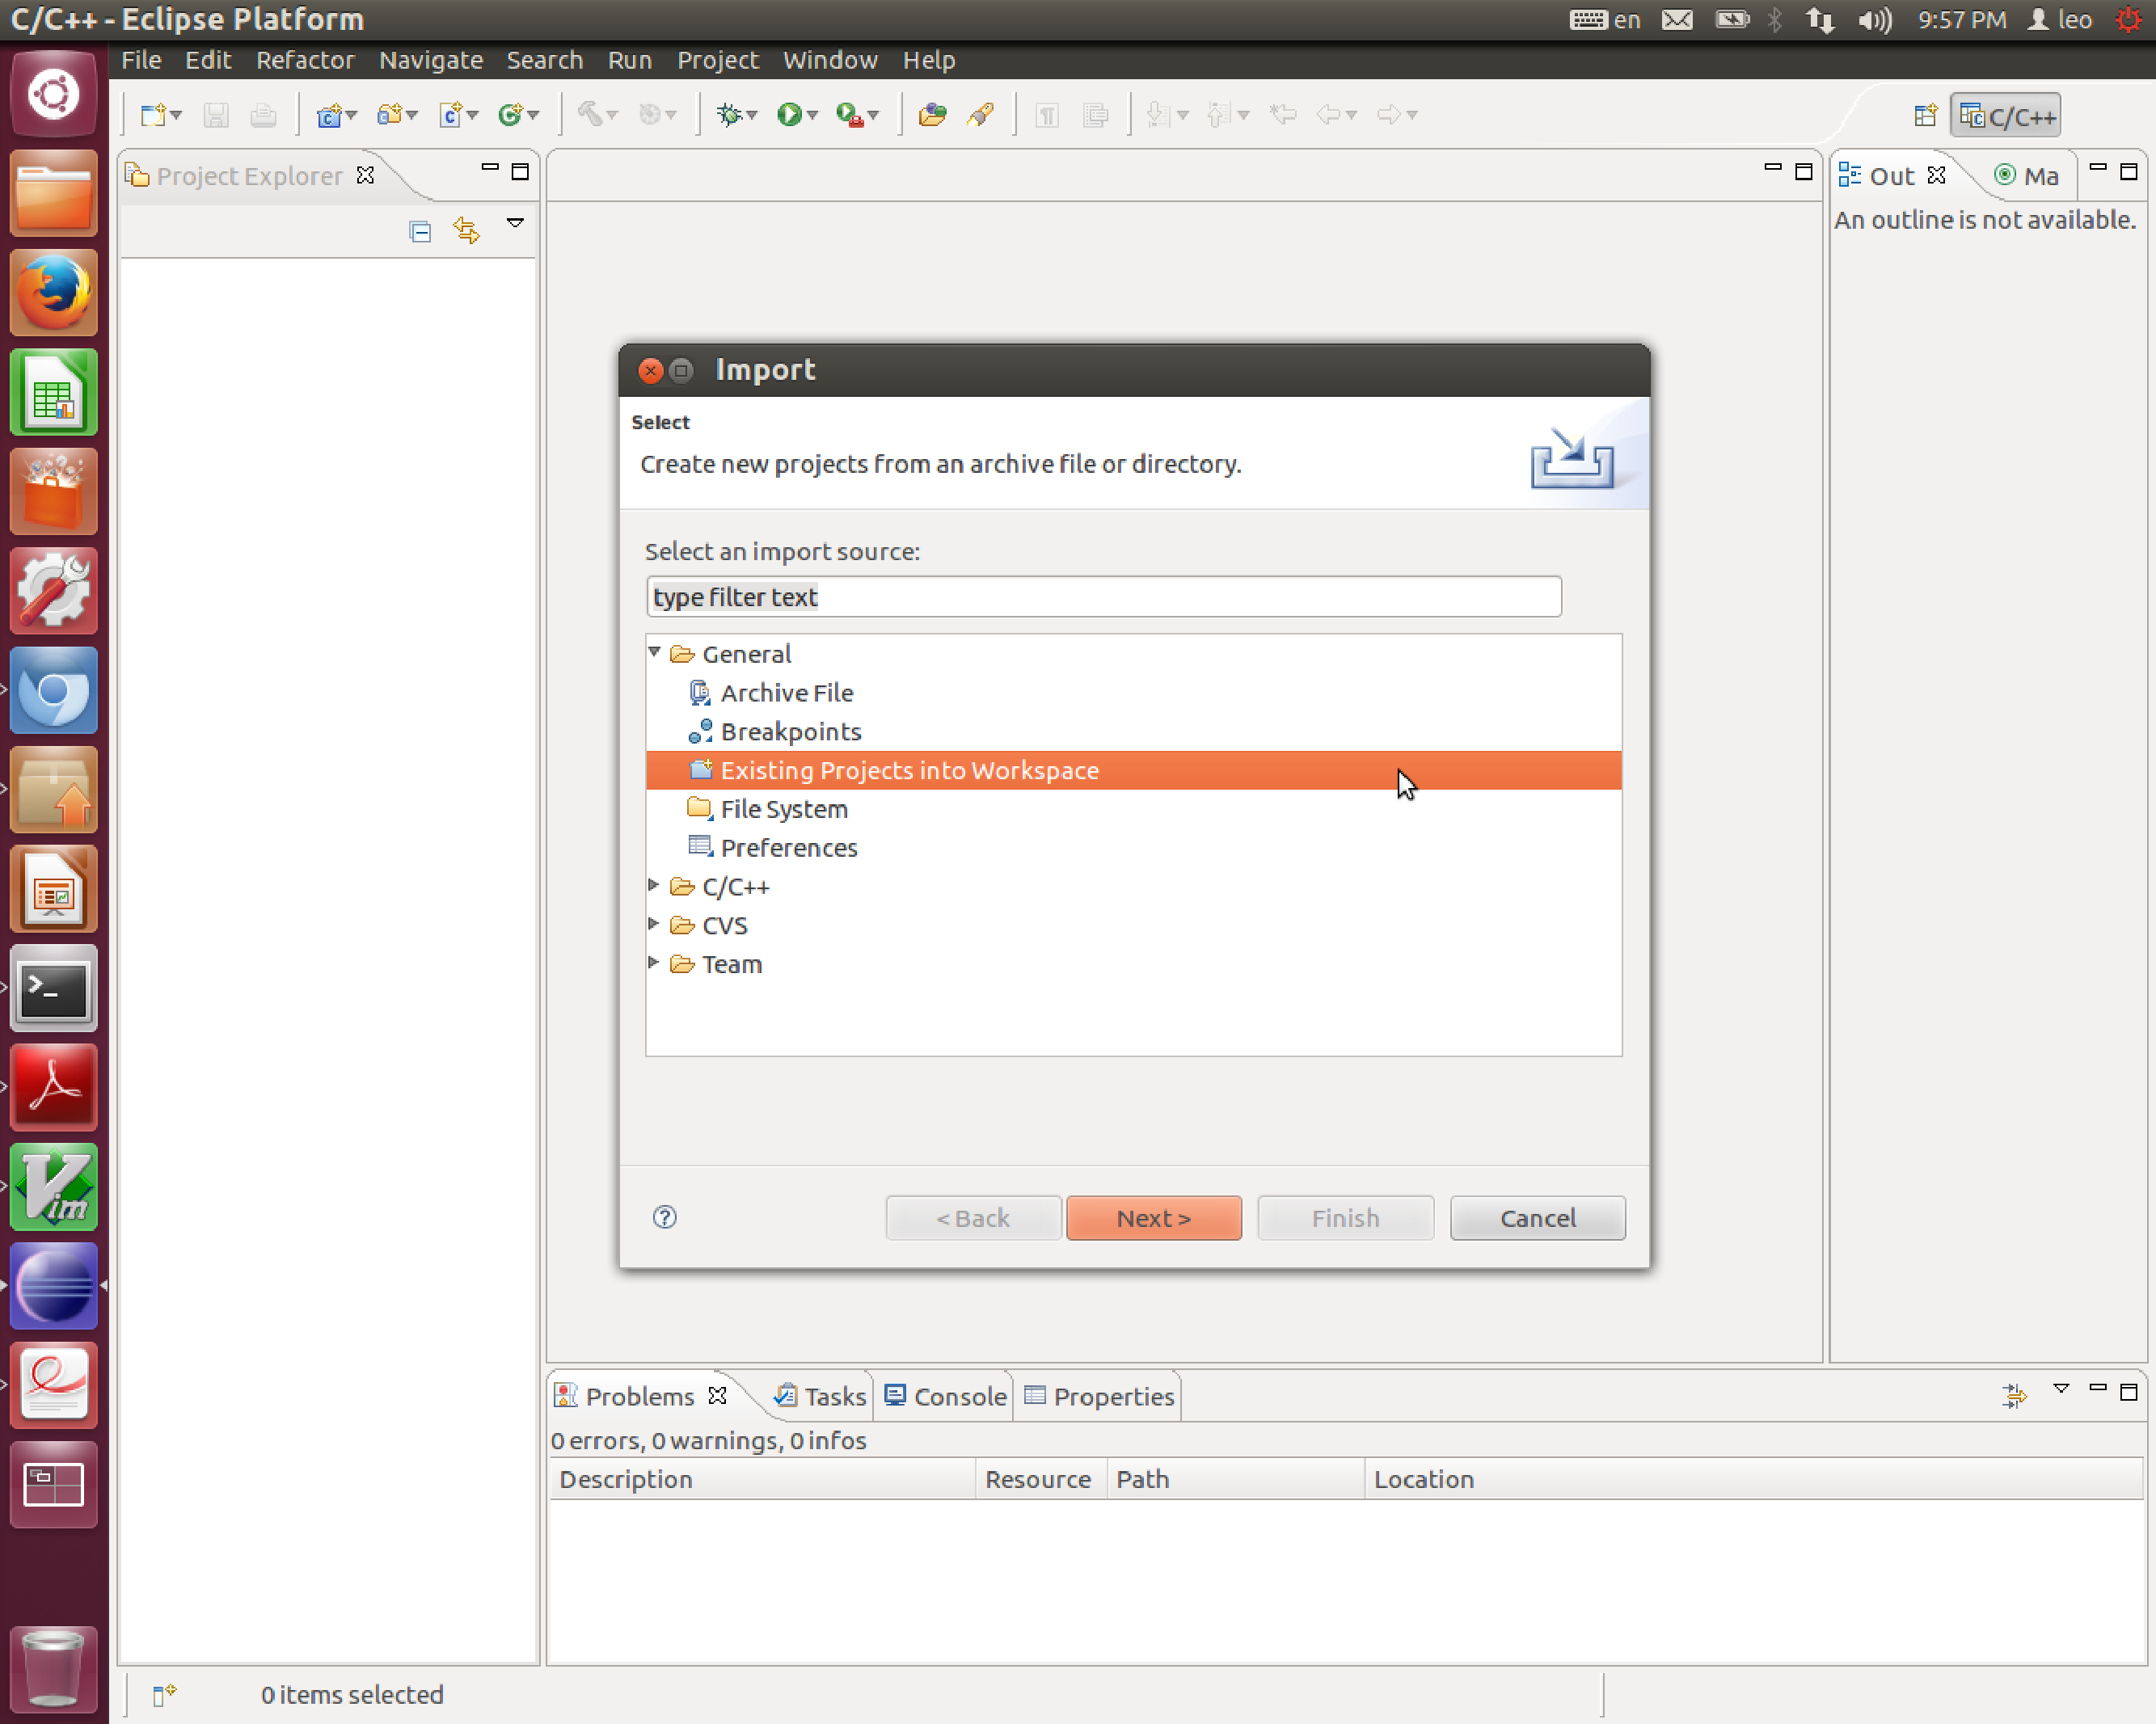
\includegraphics[width=0.9\textwidth]{figures/Eclipse1.pdf}
\end{figure}

After downloading and decompressing, e.g. as follows:
\begin{verbatim}
tar -zxvf eclipse-cpp-europa-winter-linux-gtk-x86_64.tar.gz
\end{verbatim}
one can simply run the binary \ttt{eclipse} (in a
newly created directory \ttt{eclipse}).
On the first start, Eclipse will ask you select a repository location.
This would be the place to store the project metadata and (optionally)
actual project source files.

\begin{figure}
\caption{\label{FigEclipse2}Importing an existing project}
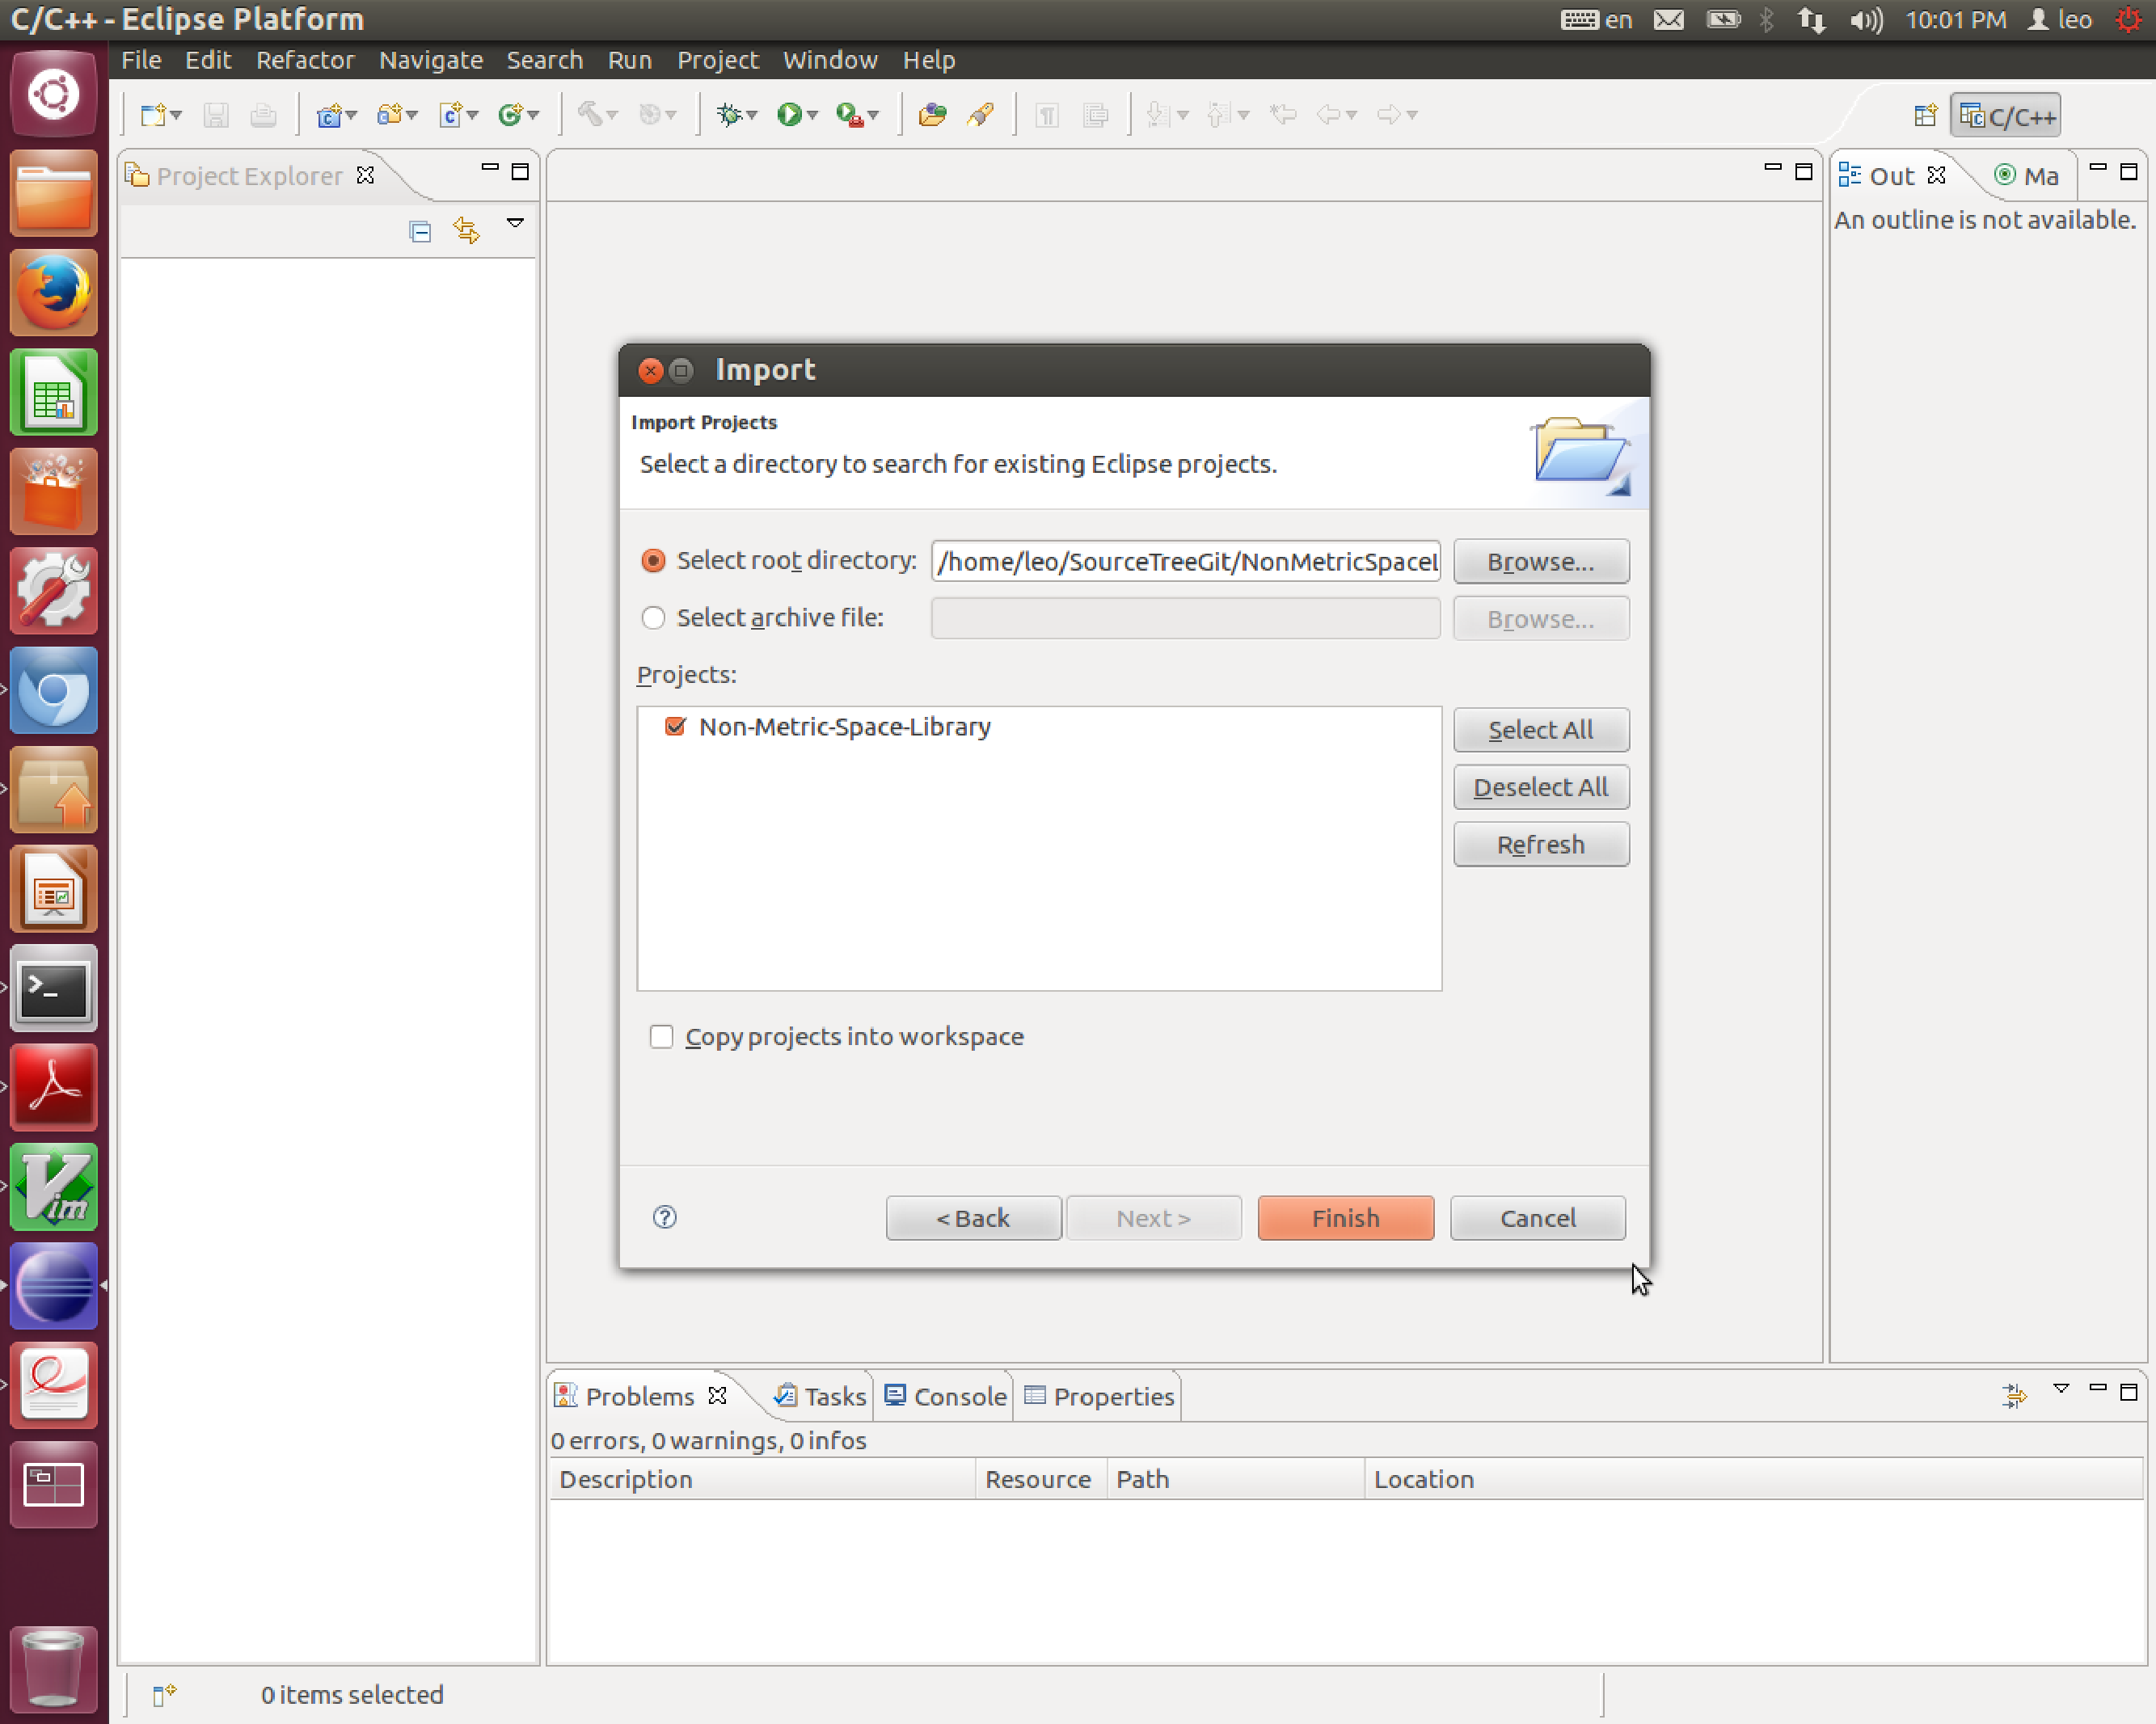
\includegraphics[width=0.9\textwidth]{figures/Eclipse2.pdf}
\end{figure}

After selecting the workspace, the user can import the Eclipse project
stored in the GitHub repository.
Go to the menu \ttt{File}, sub-menu \ttt{Import}, category \ttt{General} 
and choose to import
an existing project into the workspace as shown in Fig.~\ref{FigEclipse1}.
After that select a root directory. To this end,
go to the directory where you checked out the contents 
of the GitHub repository and enter a sub-directory \ttt{similarity\_search}.
You should now be able to see the project \ttt{Non-Metric-Space-Library}
as shown in Fig~\ref{FigEclipse2}.
You can now finalize the import by pressing the button \ttt{Finish}.

\begin{figure}
\caption{\label{FigEclipse3}Enabling indexing of the source code}
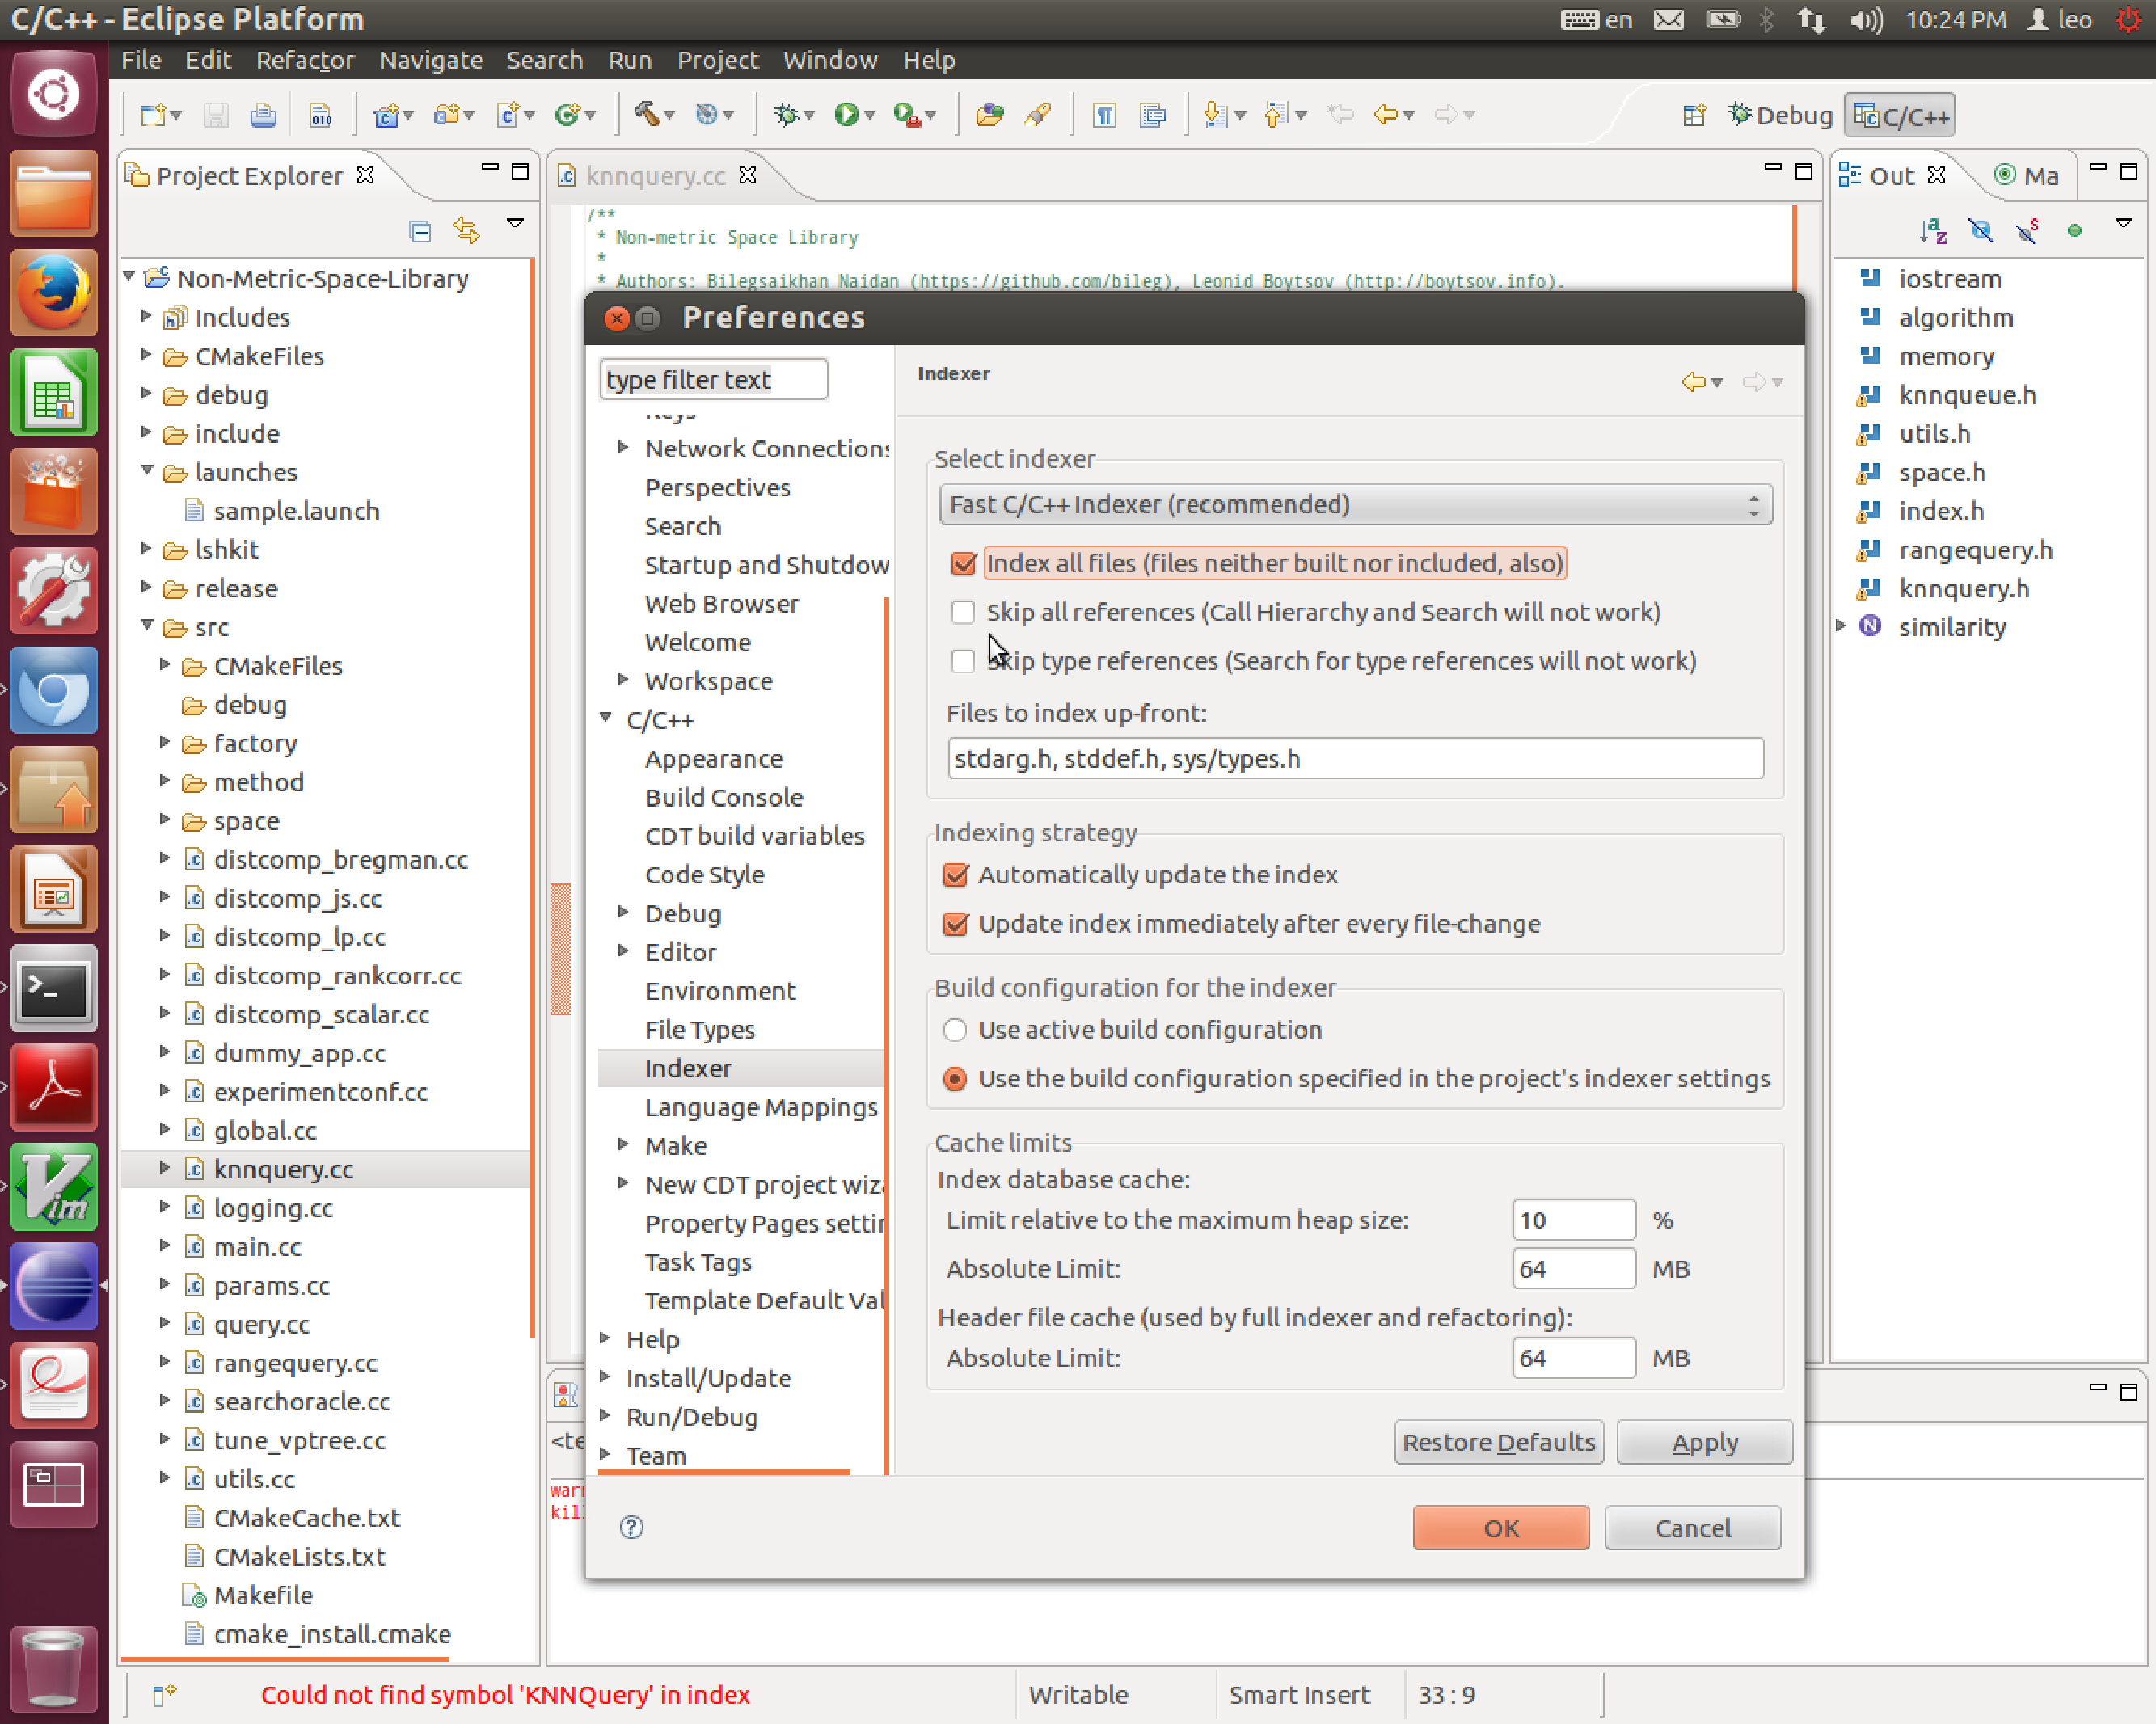
\includegraphics[width=0.9\textwidth]{figures/Eclipse3.pdf}
\end{figure}

Next, we need to set some useful settings.
Most importantly, we need to enable indexing of source files.
This would allow us to browse class hierarchies, find declarations
of variables, and classes.
To this end, go to the menu \ttt{Window}, sub-menu \ttt{Preferences}
and select a category \ttt{C++/indexing} (see Fig.~\ref{FigEclipse3}).
Then, check the box \ttt{Index all files}.
Eclipse will start indexing your files 
with the progress being shown in the status bar (right down corner).

The user can also change the editor settings. 
We would strongly encourage to disable the use of tabs.
Again, go the menu \ttt{Window}, sub-menu \ttt{Preferences}
and select a category \ttt{General/Editors/Text Editors}.
Then, check the box \ttt{Insert spaces for tabs}.
In the same menu, you can also change the fonts (use the
category \ttt{General/Appearance/Colors and Fonts}).

It is possible to build the project from Eclipse (
see the menu \texttt{Project}).
However, one first needs to generate makefiles as described in \S~\ref{SectionBuild}.
The current limitation is that you can build either release
or the debug version at a time.
Moreover, to switch from one version to another, you need to recreate
the makefiles from the command line.

\begin{figure}
\caption{\label{FigDebugConf}Creating a debug/run configuration}
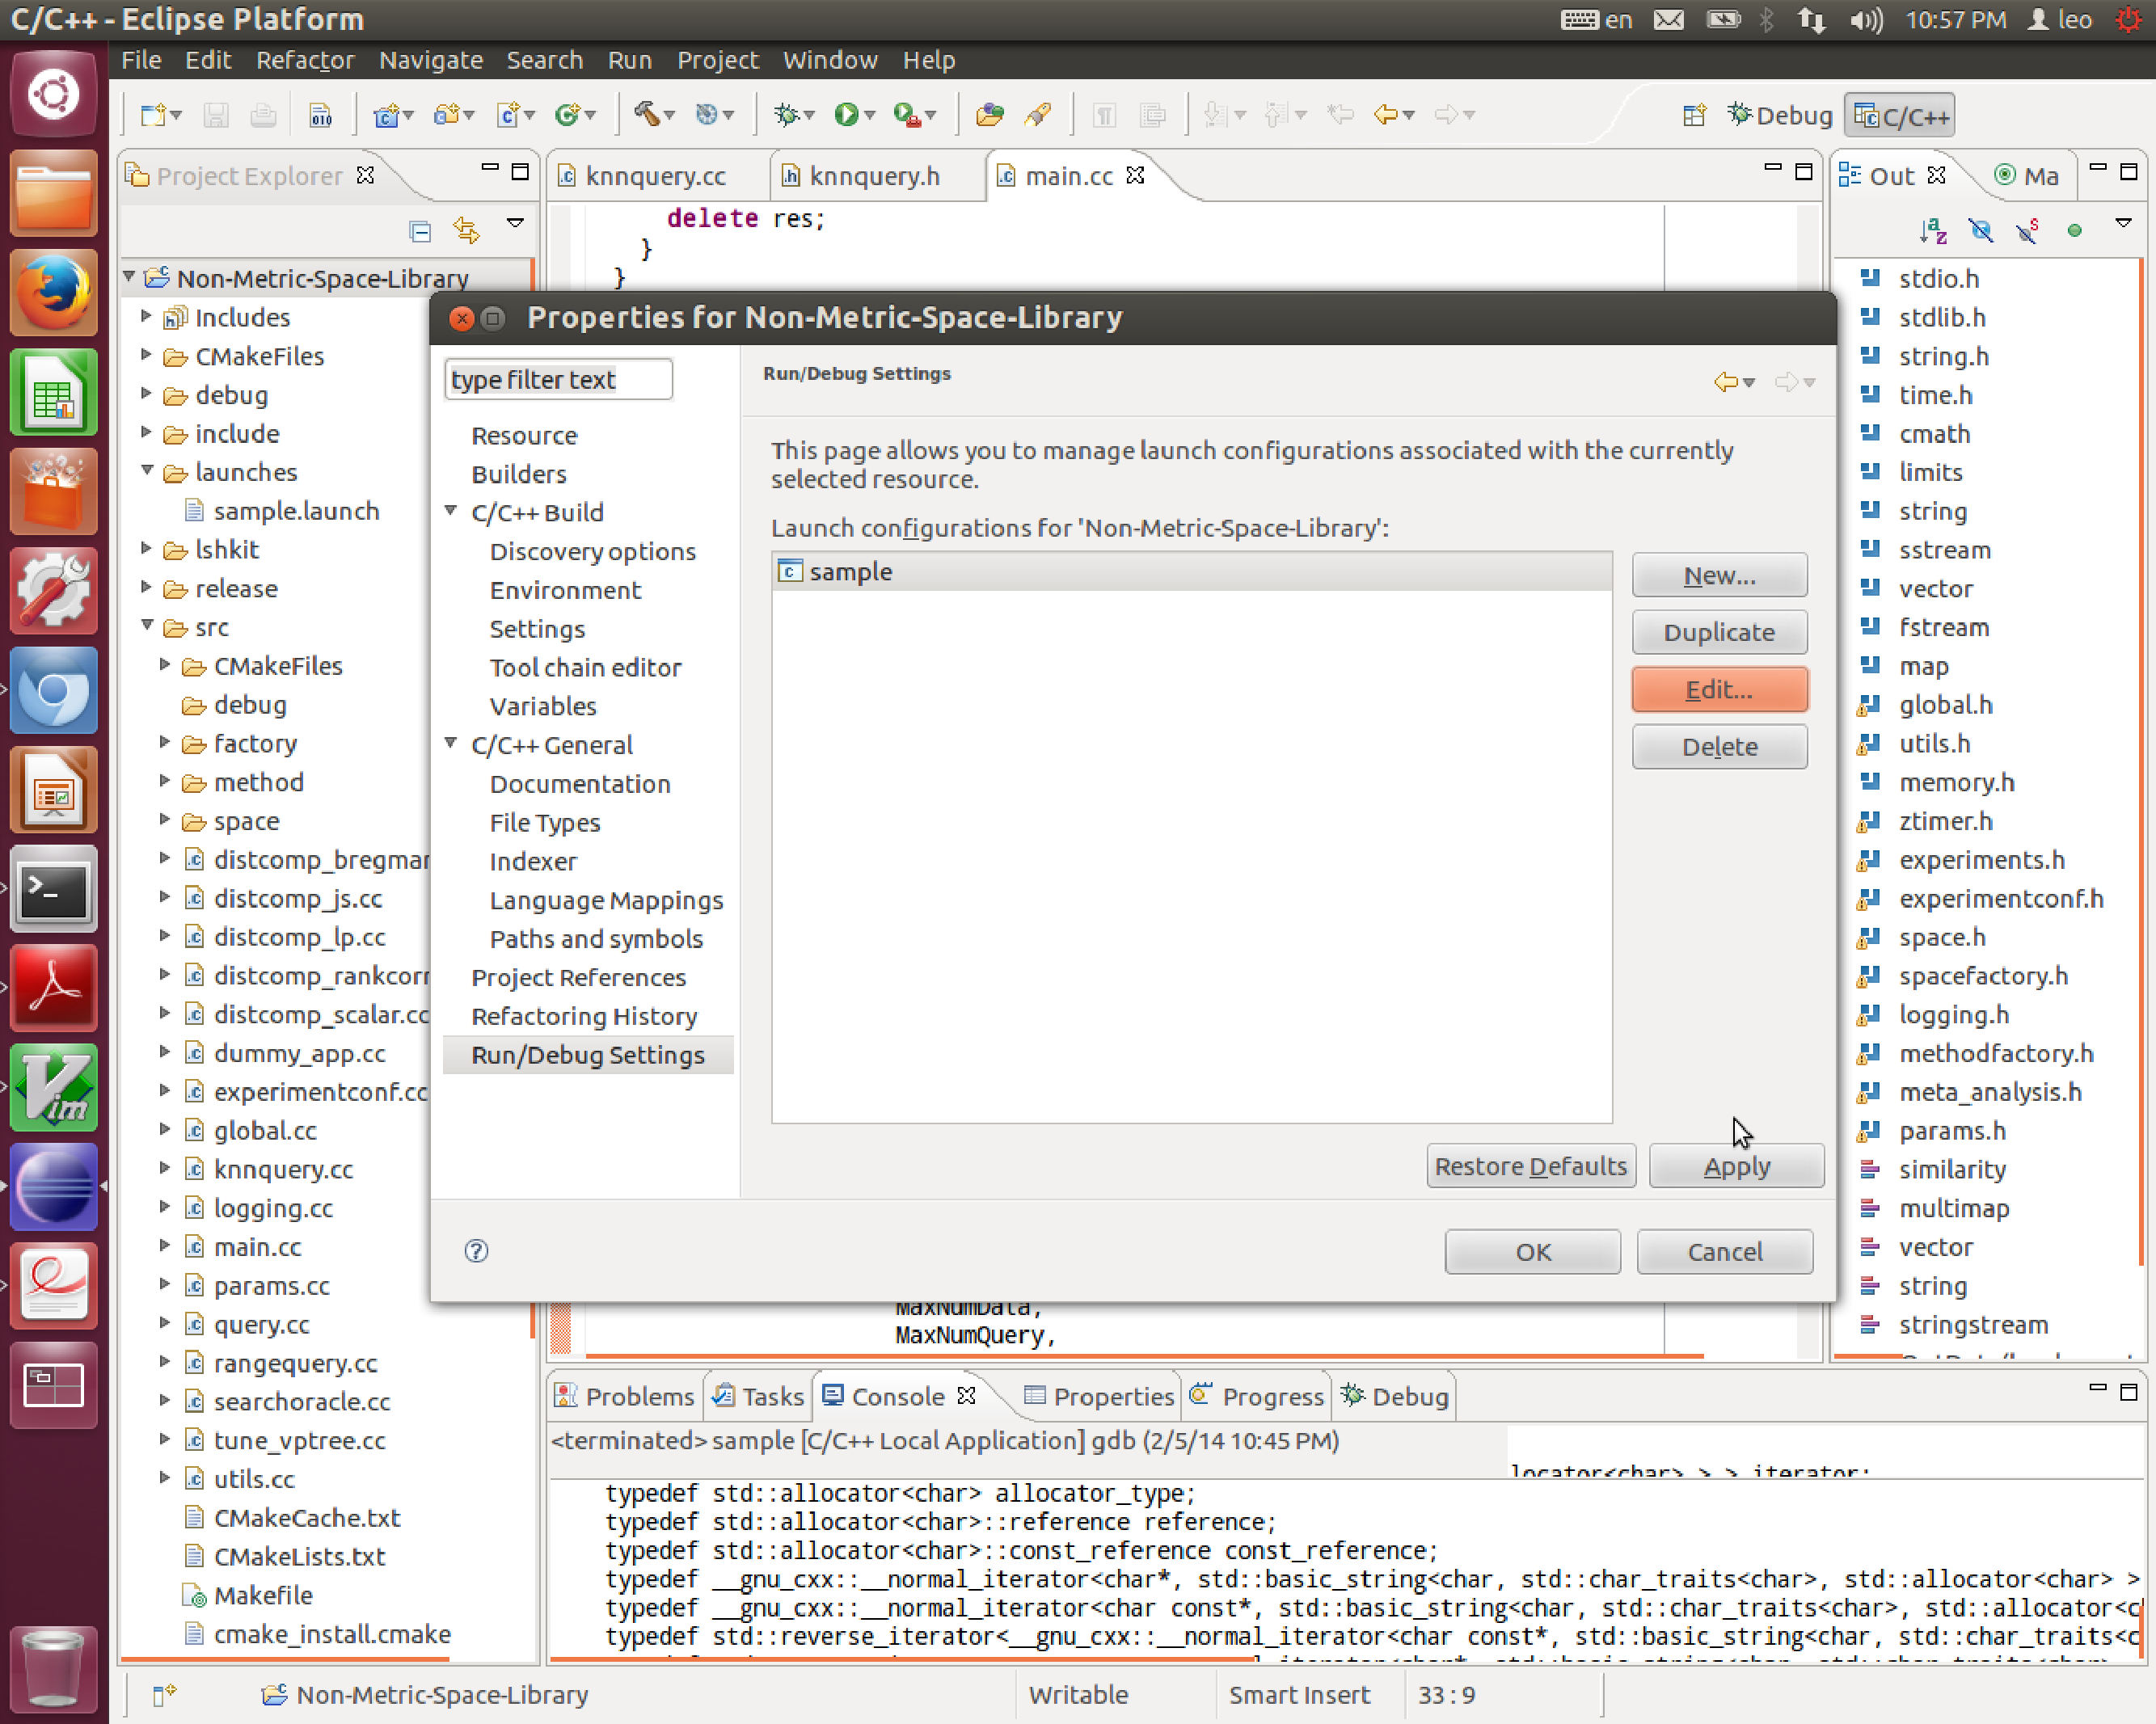
\includegraphics[width=0.9\textwidth]{figures/EclipseDebugConf.pdf}
\end{figure}

After building you can debug the project.
To do this, you need to create a debug configuration.
As an example, one configuration can be found in the 
project folder \ttt{launches}.
Right click on the item \ttt{sample.launch},
choose the option \ttt{Debug as} (in the drop-down menu),
and click on \ttt{sample} (in the pop-up menu).
After switching to a debug perspective,
the Eclipse may stop the debugger in 
the file \ttt{dl-debug.c} as shown in Fig.~\ref{FigDebug}.
If this happened, simply, press the continue icon a couple of
times until the debugger enters the code belonging to the library.

Additional configurations can be created by right clicking
on the project name (left pane), selecting \ttt{Properties}
in the pop-up menu and clicking on \ttt{Run/Debug settings}. 
The respective screenshot is shown in Fig.~\ref{FigDebugConf}.


\begin{figure}
\caption{\label{FigDebug}Starting a debugger}
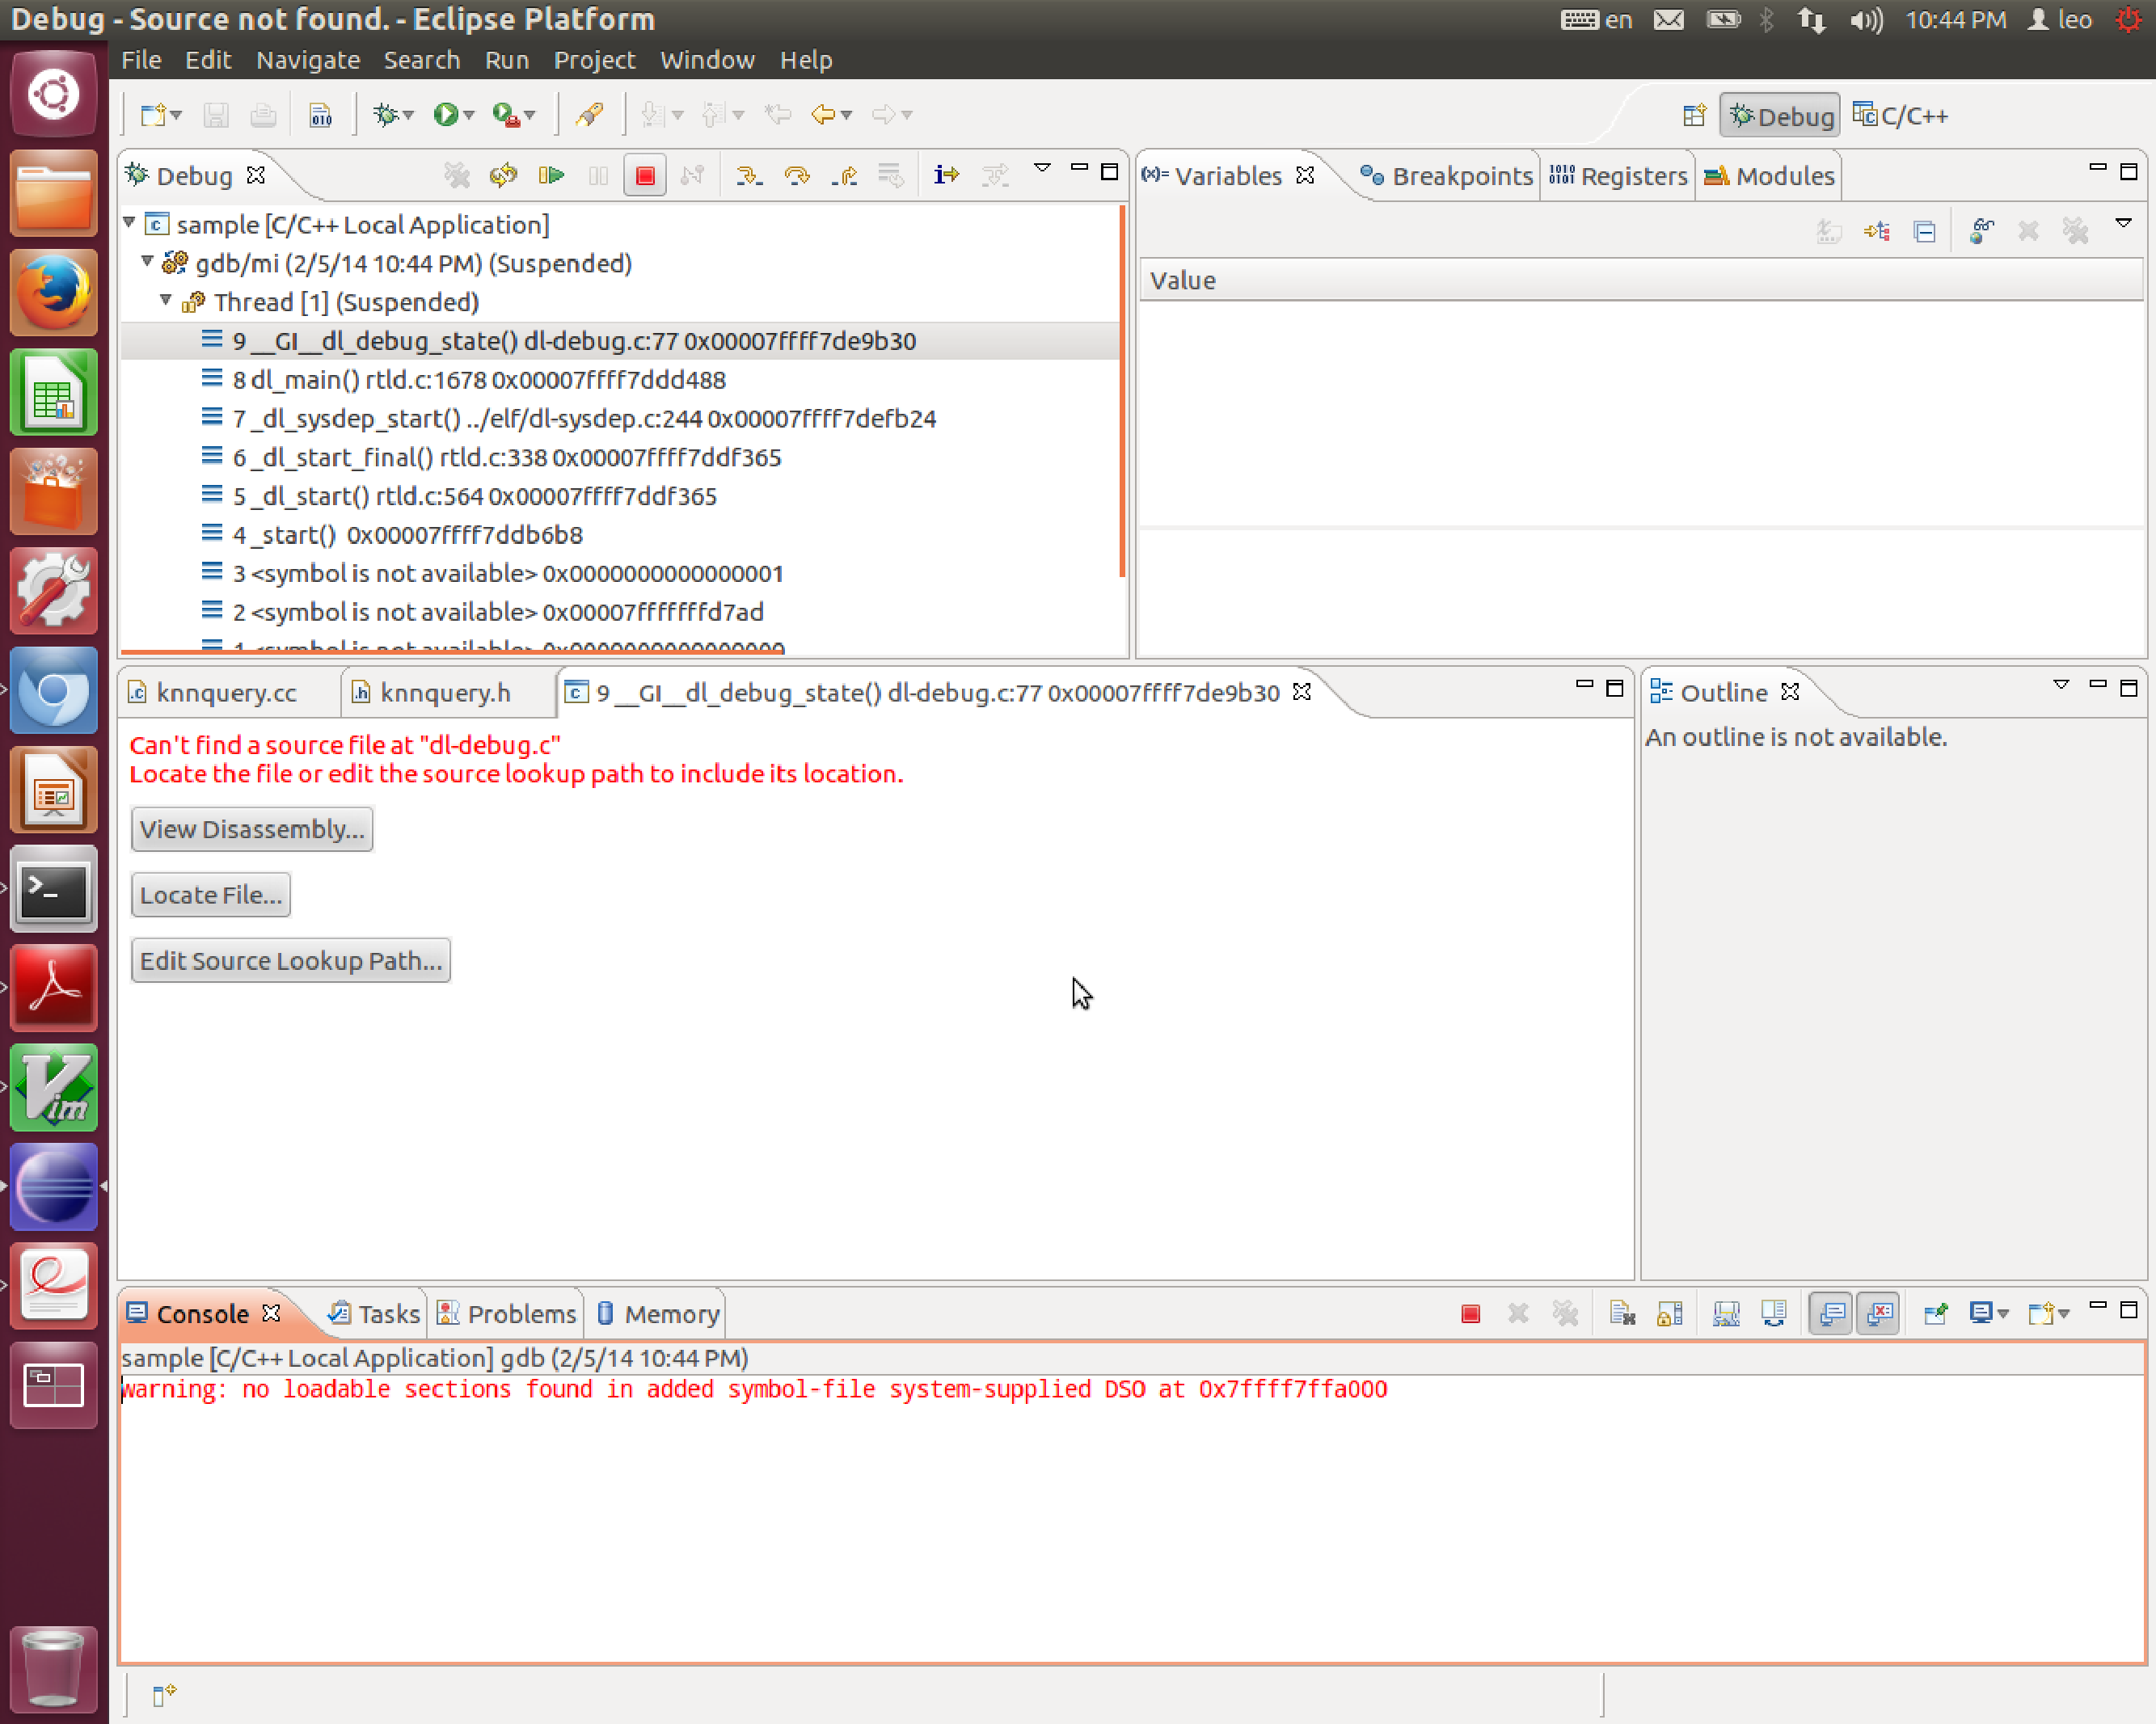
\includegraphics[width=0.9\textwidth]{figures/EclipseDebug.pdf}
\end{figure}


Note that this manual contains only a basic introduction.
If the user is new to Eclipse, we recommend reading
additional \href{http://www.eclipse.org/downloads/moreinfo/c.php}{documentation available online}.



\subsection{Running Benchmarks}\label{SectionRunBenchmark}
There is a one \ttt{single} benchmarking utility 
\ttt{experiment} that includes implementation of all methods.
It has multiple options, which specify, among others, 
a space, a data set, a type of search, and a list of methods to test (with parameters).
These options and their use cases are described in the following subsections.

\subsubsection{Space and distance value type}

A distance function can return an integer (\ttt{int}), a single-precision (\ttt{float}),
or a double-precision (\ttt{double}) real value.
A type of the distance and its value is specified as follows:

\begin{verbatim}
  -s [ --spaceType ] arg       space type, e.g., l1, l2, lp:p=0.25
  --distType arg (=float)      distance value type: 
                               int, float, double
\end{verbatim}

A description of a space may contain parameters.
In this case, there is colon after the space benchmark label followed by a
comma-separated (not spaces) list of parameters in the format:
\ttt{<parameter name>=<parameter value>}.
Currently, this is used only for $L_p$ spaces. For instance,
 \ttt{lp:0.5} denotes the space $L_{0.5}$.
A detailed list of possible spaces and respective
distance functions is given in Table~\ref{TableSpaces} in \S~\ref{SectionSpaces}.

For real-valued distance functions, one can use either single- or double-precision
type. Single-precision is a recommended default.\footnote{It is not clear yet,
if having double-precision distance functions is essential. Yet, we decided
to keep them. Thanks to C++ templates, it requires very little additional effort.}
We do not have a space with integer-valued distance function, but we
plan to implement an edit distance in the nearest future.

\subsubsection{Input Data/Test Set}
There are three options that define the data to be indexed:
\begin{verbatim}
  -i [ --dataFile ] arg        input data file
  --maxNumData arg (=0)        if non-zero, only the first 
                               maxNumData elements are used
  -d [ --dimension ] arg (=0)  optional dimensionality
\end{verbatim}
The input file can be indexed either completely, or partially.
In the latter case, the user can create the index using only
the first \ttt{--maxNumData} elements.
In the case of vector-space data, the dimensionality is determined
by the number of columns in the data file.
The user may choose to restrict the dimensionality and use only the first 
\ttt{--dimension} columns.

For testing, the user can use a separate test set.
It is, again, possible to limit the number of queries:
\begin{verbatim}
  -q [ --queryFile ] arg       query file
  --maxNumQuery arg (=1000)    if non-zero, use maxNumQuery query 
                               elements(required in the case 
                               of bootstrapping)
\end{verbatim}
If a separate test set is not available, it can be simulated by bootstrapping.
To this, end the \ttt{--maxNumData} elements of the original data set
are randomly divided into testing and indexable sets.
The number of queries in this case is defined by the option \ttt{--maxNumQuery}.
A number of bootstrap iterations is specified through an option:
\begin{verbatim}
  -b [ --testSetQty ] arg (=0) # of sets created by bootstrapping; 
\end{verbatim}
Benchmarking can be carried out in either a single- or a multi-threaded
mode. The number of test threads are specified as follows:
\begin{verbatim}
 --threadTestQty arg (=1)   # of threads
\end{verbatim}

\subsubsection{Query Type} 
Our framework supports the \knn and the range search.
The user can request to run both types of queries:
\begin{verbatim}
  -k [ --knn ] arg         comma-separated Ks for k-NN search
  -r [ --range ] arg       comma-separated values for range search
\end{verbatim}
For example, by specifying the options 
\begin{verbatim}
--knn 1,10 --range 0.01,0.1,1
\end{verbatim}
the user requests to run queries of five different types: $1$-NN, $10$-NN,
as well three range queries with radii 0.01, 0.1, and 1.

\subsubsection{Methods}
The following is an option to specify search methods:
\begin{verbatim}
  -m [ --method ] arg      list of method(s) with parameters
\end{verbatim}
Methods, similar to spaces, accept parameters. 
In this case,
the name of the method is followed by a colon and a comma-separated list (no-spaces)
of parameters in the format:
\ttt{<parameter name>=<parameter value>}.
For a detailed list of methods and their parameters, please, refer to \S~\ref{SectionMethods}.

\subsubsection{Saving and Processing Benchmark Results}
The benchmarking utility outputs a detailed report (including all the log entries) to the screen
(we plan to improve logging in the nearest future).
To save benchmarking results to a file, on needs to specify a parameter:
\begin{verbatim}
  -o [ --outFilePrefix ] arg   output file prefix
\end{verbatim}
In fact, we create two files: a human-readable report (suffix \ttt{.rep}) and 
a tab-separated data file (suffix \ttt{.data}).
By default, the benchmarking utility creates files from scratch. The
following option can be used to make it work in the append mode:
\begin{verbatim}
  --appendToResFile arg (=0)   append mode flag
\end{verbatim}
For informat

\subsection{Running Benchmarks}\label{SectionRunBenchmark}
There is a one \ttt{single} benchmarking utility 
\ttt{experiment} that includes implementation of all methods.
It has multiple options, which specify, among others, 
a space, a data set, a type of search, and a list of methods to test (with parameters).
These options and their use cases are described in the following subsections.

\subsubsection{Space and distance value type}

A distance function can return an integer (\ttt{int}), a single-precision (\ttt{float}),
or a double-precision (\ttt{double}) real value.
A type of the distance and its value is specified as follows:

\begin{verbatim}
  -s [ --spaceType ] arg       space type, e.g., l1, l2, lp:p=0.25
  --distType arg (=float)      distance value type: 
                               int, float, double
\end{verbatim}

A description of a space may contain parameters.
In this case, there is colon after the space benchmark label followed by a
comma-separated (not spaces) list of parameters in the format:
\ttt{<parameter name>=<parameter value>}.
Currently, this is used only for $L_p$ spaces. For instance,
 \ttt{lp:0.5} denotes the space $L_{0.5}$.
A detailed list of possible spaces and respective
distance functions is given in Table~\ref{TableSpaces} in \S~\ref{SectionSpaces}.

For real-valued distance functions, one can use either single- or double-precision
type. Single-precision is a recommended default.\footnote{It is not clear yet,
if having double-precision distance functions is essential. Yet, we decided
to keep them. Thanks to C++ templates, it requires very little additional effort.}
We do not have a space with integer-valued distance function, but we
plan to implement an edit distance in the nearest future.

\subsubsection{Input Data/Test Set}
There are three options that define the data to be indexed:
\begin{verbatim}
  -i [ --dataFile ] arg        input data file
  --maxNumData arg (=0)        if non-zero, only the first 
                               maxNumData elements are used
  -d [ --dimension ] arg (=0)  optional dimensionality
\end{verbatim}
The input file can be indexed either completely, or partially.
In the latter case, the user can create the index using only
the first \ttt{--maxNumData} elements.
In the case of vector-space data, the dimensionality is determined
by the number of columns in the data file.
The user may choose to restrict the dimensionality and use only the first 
\ttt{--dimension} columns.

For testing, the user can use a separate test set.
It is, again, possible to limit the number of queries:
\begin{verbatim}
  -q [ --queryFile ] arg       query file
  --maxNumQuery arg (=1000)    if non-zero, use maxNumQuery query 
                               elements(required in the case 
                               of bootstrapping)
\end{verbatim}
If a separate test set is not available, it can be simulated by bootstrapping.
To this, end the \ttt{--maxNumData} elements of the original data set
are randomly divided into testing and indexable sets.
The number of queries in this case is defined by the option \ttt{--maxNumQuery}.
A number of bootstrap iterations is specified through an option:
\begin{verbatim}
  -b [ --testSetQty ] arg (=0) # of sets created by bootstrapping; 
\end{verbatim}
Benchmarking can be carried out in either a single- or a multi-threaded
mode. The number of test threads are specified as follows:
\begin{verbatim}
 --threadTestQty arg (=1)   # of threads
\end{verbatim}

\subsubsection{Query Type} 
Our framework supports the \knn and the range search.
The user can request to run both types of queries:
\begin{verbatim}
  -k [ --knn ] arg         comma-separated Ks for k-NN search
  -r [ --range ] arg       comma-separated values for range search
\end{verbatim}
For example, by specifying the options 
\begin{verbatim}
--knn 1,10 --range 0.01,0.1,1
\end{verbatim}
the user requests to run queries of five different types: $1$-NN, $10$-NN,
as well three range queries with radii 0.01, 0.1, and 1.

\subsubsection{Methods}
The following is an option to specify search methods:
\begin{verbatim}
  -m [ --method ] arg      list of method(s) with parameters
\end{verbatim}
Methods, similar to spaces, accept parameters. 
In this case,
the name of the method is followed by a colon and a comma-separated list (no-spaces)
of parameters in the format:
\ttt{<parameter name>=<parameter value>}.
For a detailed list of methods and their parameters, please, refer to \S~\ref{SectionMethods}.

\subsubsection{Saving and Processing Benchmark Results}
The benchmarking utility outputs a detailed report (including all the log entries) to the screen
(we plan to improve logging in the nearest future).
To save benchmarking results to a file, on needs to specify a parameter:
\begin{verbatim}
  -o [ --outFilePrefix ] arg   output file prefix
\end{verbatim}
In fact, we create two files: a human-readable report (suffix \ttt{.rep}) and 
a tab-separated data file (suffix \ttt{.data}).
By default, the benchmarking utility creates files from scratch. The
following option can be used to make it work in the append mode:
\begin{verbatim}
  --appendToResFile arg (=0)   append mode flag
\end{verbatim}
For information on processing and interpreting results see \S~\ref{SectionMeasurePerf}.

\subsection{Measuring Performance and Interpreting Results}\label{SectionMeasurePerf}
\subsubsection{Efficiency}
Three types of efficiency indicators are used: query runtime, the number of distance computations,
and the amount of memory used by the index \emph{and} the data.
We also measure the improvement in runtime (improvement in efficiency) 
and in the number of distance computations compared to a sequential scan method. 
For each query, this method reads compares data objects against the query.
The sequential search baseline processes \emph{all the objects}. 

The amount of memory consumed by a search method is measured indirectly: 
We record the overall memory usage of a benchmarking process before and after creation of the index. Then, we add the amount of memory used by the data.
Memory used is computed by querying special file \ttt{/dev/<process id>/status}. 
This works only for Linux as we do not have a portable code to measure memory consumption of a process.

\subsubsection{Effectiveness}

Several effectiveness metrics are computed by the benchmarking utility:
\begin{itemize}
\item  A \emph{number of points closer} to the query than the nearest returned point.
Let $\pos(o_i)$ represent a positional distance from $o_i$ to the query, 
i.e., the number of objects closer to the query than $o_i$ plus one.
In the case of ties, we assume that the object with a smaller index is closer to the query.
Note that $\pos(o_i) \ge i$.
\item A \emph{relative position} error is equal to $\pos(o_i)/i$;
\item \emph{Recall},  which is is equal to the fraction of all correct answers retrieved.
\end{itemize}
The first two metrics represent a so-called rank (approximation) error:
if we sort (i.e., rank) all the data objects with respect to their distances to the query,
where do we place objects returned by the search method?
The closer the returned objects are to the beginning of the list (i.e., 
the closer they are to to the query object), the better is the quality of the search response.

Recall is a classic metric. 
It was argued, however, 
that recall does not account for position information of returned objects
and is, therefore, inferior to rank error metrics \cite{Amato_et_al:2003,Cayton:2008}.
If we had ground-truth queries and relevance judgements from human assessors (e.g.,
if a vector represents an image, it is similar to the query image?),
we could in principle compute even more realistic effectiveness metrics 
such as the mean average precision,
or the normalized discounted cumulative gain.
This remains for the future work.

\subsection{Interpreting and Processing Benchmark Results}
If the user specifies the option \ttt{--outFilePrefix},
the benchmarking results are saved to two files:
the file in a human-readable format,
and a tab-separated data file intended for automatic processing.

\begin{wraptable}{R}{0.52\textwidth}
\caption{An example of a human-readable report 
\label{TableHRep}}
\begin{verbatim}
===================================
vptree: triangle inequality
===================================
# of points: 9900
# of queries: 100
------------------------------------
Recall:        0.83 -> [0.756 0.903]
RelPosError:   1.33 -> [1.14   1.55]
NumCloser:     2.05 -> [-0.11  4.21]
------------------------------------
QueryTime:     2.04 -> [1.62   2.46]
DistComp:      472 ->  [1963  2981]
------------------------------------
ImprEfficiency:3.97 -> [3.97   3.97]
ImprDistComp:  4    -> [4   4]
------------------------------------
Memory Usage:  8.48 MB
------------------------------------
\end{verbatim}
\textbf{Note:} \emph{confidence intervals} are in brackets
\vspace{-4em}
\end{wraptable}

The data file contains only the average values,
which can be used to, e.g., produce efficiency-effectiveness plots.
A sample script for doing this so can be found in the \href{https://github.com/searchivarius/NonMetricSpaceLib/blob/master/sample_scripts/nips2013/figures/all.sh}{sample\_scripts} directory.
The human-readable report also provides 95\% confidence intervals.
In the case of bootstrapping, statistics collected from several iterations,
are aggregated using a classic fixed-effect model adopted in meta analysis \cite{Hedges_and_Vevea:1998}.
Note for all metrics, except relative error, an average is computed using an arithmetic mean.
For the relative error, however, we use the geometric mean  \cite{king:1986}.

An example of human readable report (\emph{confidence intervals} are in square brackets)
is given in Table~\ref{TableHRep}.

%\newpage
\section{Spaces}\label{SectionSpaces}
Currently we support only vector spaces.
The input files can come in either regular, i.e., dense,
or sparse variant. 
In both cases vectors are stored
as a plain-text file, one vector per row.
Yet, the vector formats are different.

In the regular, dense-vector, format, each row
contains the same number of vector elements, one per each dimension.
The values can be separated by spaces or commas/columns.
In the sparse format, each vector elements is preceded
by a \emph{zero-based} vector element id. 
The ids can be unsorted, but they should not repeat.
For example, the following line
describes a vector with three explicitly specified values,
which represent vector elements 0, 25, and 257:
\begin{verbatim}
0 1.234  25 0.03 257 -3.4 
\end{verbatim}

Most values are missing and are assumed to have a default value.
It is up to a designer of the space to decide on the default.
Yet, all current implementations choose the \emph{zero} default value.
Again, elements can be separated by spaces or commas/columns instead of spaces.

For a detailed list of spaces, their parameters, 
and performance characteristics is given in Table~\ref{TableSpaces}.
The label of the space is passed to the benchmarking utility (see \S~\ref{SectionRunBenchmark}).
There can be more than one version of a distance function,
which have different space-performance trade-off.
In particular, for distances that require computation of logarithms 
we can achieve an order of magnitude improvement (for the GNU C++) by precomputing
logarithms at index time. This comes at a price of extra storage. 
In the case of Jensen-Shannon distance functions, we can pre-compute some 
of the logarithms and accurately approximate those we cannot pre-compute.
The details are explained in \S~\ref{SectionLP}-\ref{SectionBregman}.

Straightforward slow implementations of the distance functions may have the substring \ttt{slow}
in their names, while faster versions contain the substring \ttt{fast}.
Fast functions that involve approximate computations contain additionally the substring \ttt{approx}.
For non-symmetric distance function, a space may have two variants: one variant is for left
queries (the query object is the first argument of the distance function) 
and another is for right queries (the query object is the second argument).
In the latter case the name of the space ends on \texttt{rq}.
Separating spaces by query types, might not be the best approach.
Yet, it seems to be unavoidable, because, in many cases,
we need separate indices for left and right queries.

Distance computation efficiency was evaluated on a Core i7 laptop (3.4 Ghz peak frequency)
in a single-threaded mode (by the utility \href{https://github.com/searchivarius/NonMetricSpaceLib/blob/master/similarity_search/test/bunit.cc}{bunit}).
It is measured in millions of computations per second for single-precision
floating pointer numbers (double precision computations are, of course, more costly). 
The code was computed using the GNU compiler. 
Somewhat higher efficiency numbers can be obtained by using the Intel compiler.
In fact, performance is much better for distances relying on ``heavy'' math functions:
slow versions of KL- and Jensen-Shannon divergences and Jensen-Shannon metrics, 
as well as for $L_p$ spaces,
where $p \not\in\{1,2,\infty\}$.

In the efficiency test, all dense vectors have 128 elements.
For all dense-vector distances except the Jensen-Shannon divergence,
their elements were generated randomly and uniformly.
For the Jensen-Shannon divergence, we first generate elements randomly,
and next we randomly select elements that are set to zero (approximately half). 
Additionally, for KL-divergences and the JS-divergence,
we normalize vector elements so that they correspond a true discrete probability distribution. 
Sparse space distances were tested using sparse vectors from a small sample file in the
\href{https://github.com/searchivarius/NonMetricSpaceLib/blob/master/sample_data/sparse_5K.txt}{sample\_data} directory.

\hspace{-2em}\begin{table}
\caption{Description of implemented spaces\label{TableSpaces}}
\centering
\begin{tabular}{l@{\hspace{2mm}}l@{\hspace{2mm}}l}
\toprule
\textbf{Space}& \textbf{Label\&Formula}   & \textbf{Efficiency} \\
              &                           & (million op/sec) \\
\toprule
\multicolumn{3}{c}{\textbf{Metric Spaces}}  \\
\toprule
Hamming &  \ttt{bit\_hamming}                      &  240 \\
                 &  $\sum_{i=1}^n |x_i-y_i|$                         &  \\
\cmidrule(l){1-3} 
$L_1$     &  \ttt{l1}, \ttt{l1\_sparse}              &                   35, 1.6 \\
                 &  $\sum_{i=1}^n |x_i-y_i|$                         &  \\
\cmidrule(l){1-3} 
$L_2$     &  \ttt{l2}, \ttt{l2\_sparse}              &                  30, 1.6  \\
                 & $\sqrt{\sum_{i=1}^n |x_i-y_i|^2}$                 &   \\
\cmidrule(l){1-3} 
$L_{\infty}$ &  \ttt{linf}, \ttt{linf\_sparse}      &   34 , 1.6  \\
                    & $\max_{i=1}^n |x_i-y_i|$           & \\
\cmidrule(l){1-3} 
$L_p$ (generic $p \ge 1$)& \ttt{lp:p=\ldots}, \ttt{lp\_sparse:p=\ldots}  &  0.1-3, 0.1-1.2  \\
                                & $\left(\sum_{i=1}^n |x_i-y_i|^p\right)^{1/p}$  & \\
\cmidrule(l){1-3} 
Angular distance & \ttt{angulardist}, \ttt{angulardist\_sparse} & { 13, 1.4 } \\
                        & $\arccos\left(1-\frac{\sum_{i=1}^n x_i y_i}{\sqrt{\sum_{i=1}^n x_i^2}\sqrt{\sum_{i=1}^n y_i^2 }}\right)$   & \\
\cmidrule(l){1-3} 
Jensen-Shan. metr. &\ttt{jsmetrslow, jsmetrfast, jsmetrfastapprox} &  0.3, 1.9, 4.8  \\
                          & $\sqrt{\frac{1}{2}\sum_{i=1}^n \left[x_i \log x_i + y_i \log y_i  - (x_i+y_i)\log \frac{x_i +y_i}{2}\right]}$  & \vspace{1em} \\
\toprule
\multicolumn{3}{c}{\textbf{Non-metric spaces (symmetric distance)}}  \\
\toprule
$L_p$ (generic $p < 1$)& \ttt{lp:p=\ldots, lp\_sparse:p=\ldots}                     &  0.1-3, 0.1-1 \\
                              & $\left(\sum_{i=1}^n |x_i-y_i|^p\right)^{1/p}$  &   \\
\cmidrule(l){1-3} 
Jensen-Shan. div. &\ttt{jsdivslow, jsdivfast, jsdivfastapprox} &   0.3, 1.9, 4.8 \\
                          & $\frac{1}{2}\sum_{i=1}^n \left[x_i \log x_i + y_i \log y_i  - (x_i+y_i)\log \frac{x_i +y_i}{2}\right]$ & \\
\cmidrule(l){1-3} 
Cosine similarity & \ttt{cosinesimil}, \ttt{cosinesimil\_sparse} & { 13, 1.4 } \\
                        & $1-\frac{\sum_{i=1}^n x_i y_i}{\sqrt{\sum_{i=1}^n x_i^2}\sqrt{\sum_{i=1}^n y_i^2 }}$   & \vspace{1em} \\
\toprule
\multicolumn{3}{c}{\textbf{Non-metric spaces (non-symmetric distance)}}  \\
\toprule
regular KL-div. & left queries: \ttt{kldivfast}       & 0.5, 27 \\
                       & right queries: \ttt{kldivfastrq}    &  \\
                       & $\sum_{i=1}^n   x_i \log \frac{x_i}{y_i}$  & \\ 
\cmidrule(l){1-3} 
generalized KL-div. & left queries: \ttt{kldivgenslow}, \ttt{kldivgenfast} & 0.5, 27    \\
                           & right queries: \ttt{kldivgenfastrq} & 27    \\
                           & $\sum_{i=1}^n \left[  x_i \log \frac{x_i}{y_i} -   x_i +   y_i \right]$   &   \\
\cmidrule(l){1-3} 
Itakura-Saito & left queries: \ttt{itakurasaitoslow, itakurasaitofast}   & 0.2, 3, 14 \\
              & right queries: \ttt{itakurasaitofastrq}                  & 14         \\
              & $\sum_{i=1}^n \left[ \frac{ x_i}{y_i} - \log \frac{x_i}{y_i}  -1 \right]$ \\
\toprule
\end{tabular}
\end{table}

\subsection{$L_p$-norms}\label{SectionLP}
The $L_p$ distance between vectors $x$ and $y$ are
given by the formula:
\begin{equation}\label{EqMink}
L_p(x,y) = \left(\sum_{i=1}^n |x_i-y_i|^p\right)^{1/p}
\end{equation}
In the limit ($p \rightarrow \infty$),
the $L_p$ distance becomes the Maximum metric, also known as 
the Chebyshev distance:
\begin{equation}\label{EqCheb}
L_{\infty}(x,y) = \max\limits_{i=1}^n |x_i-y_i|
\end{equation}
$L_{\infty}$ and all spaces $L_p$ for $p \ge 1$
are true metrics. 
They are symmetric, equal to zero only for identical elements,
and, most importantly, satisfy \emph{the triangle inequality}.
However, the $L_p$ norm is \emph{not} a metric if $p<1$.

In the case of dense vectors, 
we have reasonably efficient implementations 
for $L_p$ distances where $p$ is either integer or infinity. 
The most efficient implementations are for $L_1$ (Manhattan),
$L_2$ (Euclidean), and $L_{\infty}$ (Chebyshev).
As explained in Leo's blog,
\href{http://searchivarius.org/blog/efficient-exponentiation-square-rooting}{we compute exponents through square rooting}. 
This works best when the number of digits (after the binary digit) is small, e.g., if $p=0.125$.

Any $L_p$ space can have a dense and a sparse variant.
Sparse vector spaces have their own labels, which are different
from dense-space labels in that they contain a suffix \ttt{\_sparse} (see also Table~\ref{TableSpaces}).
For instance \texttt{l1} and \texttt{l1\_sparse} are both $L_1$ spaces,
but the former is dense and the latter is sparse.
The labels of $L_1$, $L_2$, and $L_\infty$ spaces (passed to the benchmarking utility) are
\ttt{l1}, \ttt{l2}, and \ttt{linf}, respectively.
Other generic $L_p$ have the name $lp$, which is used in combination with a parameter.
For instance, $L_3$ is denoted as \ttt{lp:p=3}.

Distance functions for sparse-vector spaces are far less efficient, 
due to a costly, branch-heavy, operation of matching sparse vector indices
(between two sparse vectors).

\subsection{Scalar-product Related Distances}
We have two distance function whose formulas include normalized scalar product.
One is the cosine similarity, which is equal to:
$$
d(x,y) =1-\frac{\sum_{i=1}^n x_i y_i} 
{\sqrt{\sum_{i=1}^n x_i^2} \sqrt{\sum_{i=1}^n y_i^2 } } 
$$ 
The cosine similarity is not a true metric, but it can be converted into
one by applying a monotonic transformation (i.e.., taking an inverse cosine).
The resulting distance function is a true metric that 
is called the angular distance.
The angular distance is computed using the following formula:
$$
d(x,y) =\arccos\left(1-\frac{\sum_{i=1}^n x_i y_i} 
{\sqrt{\sum_{i=1}^n x_i^2} \sqrt{\sum_{i=1}^n y_i^2 } }\right) 
$$ 

\subsubsection{Jensen-Shannon divergence}\label{SectionJS}
\emph{Jensen-Shannon} divergence is a symmetrized and smoothed KL-divergence:
\begin{equation}\label{EqJS}
\frac{1}{2}\sum_{i=1}^n\left[ x_i \log x_i + y_i \log y_i  -(x_i+y_i)\log \frac{x_i +y_i}{2}\right]
\end{equation}
This divergence is symmetric, but it is not a metric function.
However, the square root of the Jensen-Shannon divergence
is a proper a metric \cite{endres2003new},
which we call the Jensen-Shannon metric.

A straightforward implementation of Eq.~\ref{EqJS} is inefficient for two reasons 
(at least when one uses the GNU C++ compiler)
(1) computation of logarithms is a slow operation (2)
the case of zero $x_i$ and/or $y_i$ requires conditional processing, i.e.,
costly branches.

A better method is to pre-compute logarithms of data at index time. 
It is also necessary to compute logarithms of a query vector.
However, this operation has a little cost since it is carried out once 
for each nearest neighbor or range query.
Pre-computation leads to a 3-10 fold improvement depending on the sparsity of vectors,
albeit at the expense of requiring twice as much space.
Unfortunately, it is not possible to avoid computation of the third logarithm:
it needs to be computed in points that are not known until we see the query vector.

However, it is possible to approximate it with a very good precision,
which should be sufficient for the purpose of approximate searching.
To this end, we rewrite the equation \ref{EqJS} as follows:
$$
\frac{1}{2}\sum_{i=1}^n\left[ x_i \log x_i + y_i \log y_i  -(x_i+y_i)\log \frac{x_i +y_i}{2}\right]=
$$
$$
 = \frac{1}{2}\sum_{i=1}^n\left[ x_i \log x_i + y_i \log y_i\right]  -
\sum_{i=1}^n\left[\frac{(x_i+y_i)}{2}\log \frac{x_i +y_i}{2} \right]=
$$
$$
 = \frac{1}{2}\sum_{i=1}^n x_i \log x_i + y_i \log y_i  -
$$
\begin{equation}\label{Eq1}
\sum_{i=1}^n\frac{(x_i+y_i)}{2}\left[\log\frac{1}{2} + \log \max(x_i,y_i) + 
\log \left(1 + \frac{\min(x_i,y_i)}{\max(x_i,y_i)}\right) \right]
\end{equation}
We can pre-compute all the logarithms in Eq.~\ref{Eq1} except for $\log \left(1 + \frac{\min(x_i,y_i)}{\max(x_i,y_i)}\right) $. However, its argument value is in a small range: from one to two.
We can discretize the range, compute logarithms in many intermediate points and save the computed values in a table.
Finally, we employ the SIMD operations to implement this approach. 
As our tests show, this is a very efficient approach, which results in a very little (around $10^{-6}$ on average) relative error for the value of the Jensen-Shannon divergence.

Another possible approach is use \href{http://fastapprox.googlecode.com/svn/trunk/fastapprox/src/fastonebigheader.h}{an efficient approximation for logarithm computation}.
However, \href{https://github.com/searchivarius/BlogCode/tree/master/2013/12/26}{as our tests show},
this method is still relatively slow (it takes almost 20 CPU cycles per log),
 while the relative error is as high as $3 \cdot 10^{-4}$ for logarithm arguments smaller than 2.

\subsection{Bregman Divergences}\label{SectionBregman}
Bregman divergences are typically non-metric distance functions,
which are equal to a difference between some convex differentiable function $f$
and its first-order Taylor expansion \cite{Bregman:1967,Cayton:2008}. 
More formally, given the convex and differentiable function $f$
(of many variables), its
corresponding Bregman divergence $d_f(x,y)$ is equal to:
$$
d_f(x,y) = f(x) - f(y) - \langle\nabla f(y), x - y \rangle
$$
where $\langle x,y\rangle$ denotes the scalar product of vectors $x$ and $y$.
In this library, we implement the generalized KL-divergence 
and the Itakura-Saito divergence,
which correspond to functions $f=\sum x_i \log x_i - \sum x_i$ and $f = - \sum \log x_i$. 
The generalized KL-divergence is equal to:
$$
\sum_{i=1}^n \left[  x_i \log \frac{x_i}{y_i} -   x_i +   y_i \right],
$$
while the Itakura-Saito divergence is equal to:
$$ 
\sum_{i=1}^n \left[ \frac{ x_i}{y_i} - \log \frac{x_i}{y_i}  -1 \right].
$$
If vectors $x$ and $y$ are proper probability distributions, $\sum x_i = \sum y_i = 1$.
In this case, the generalized KL-divergence becomes a regular KL-divergence:
$$
\sum_{i=1}^n \left[  x_i \log \frac{x_i}{y_i} \right].
$$

Computing logarithms is costly: We can considerably improve efficiency of 
evaluation Itakura-Saito divergence and KL-divergence by pre-computing logarithms at index time.
The spaces that implement this functionality contain the substring \ttt{fast} in their labels (see also Table~\ref{TableSpaces}).


\section{Search Methods}\label{SectionMethods}
Implemented search methods can be broadly divided into the following 
categories:
\begin{itemize}
\item Pivoting and compact partitioning methods for metric spaces \cite{Chavez_et_al:2001a};
\item Filtering methods based on permutations;
\item Filtering methods based on random projections;
\item A specialized method (bbtree) for Bregman divergences \cite{Cayton:2008};
\item A vantage-point tree (a VP-tree) with pluggable search oracles, 
which can be used in both metric and non-metric spaces.
\end{itemize}

Pivoting methods rely on embedding into a vector space with the $L_{\infty}$ distance.
Partitioning is based on how far (or close) the data points are located with respect to pivots.
If the original space is a metric spacing such an embedding is contractive:
The $L_{\infty}$ distance in the target vector space is a lower bound for the original distance.

Hierarchical partitions produced by pivoting methods lack locality: a single partition can contain
far away data points. Compact partitioning schemes exploit locality.
They either divide the data into clusters or use a Voronoi partitioning (or its approximation).
In the latter case, for example, we can select several centers/pivots $\pi_i$ and associate 
data points with the closest center.

These classic search methods are exact. It is possible to convert most of them to approximate
methods using an early termination technique,
where we terminate the search after exploring a sufficient number of data points.
The data points are often grouped into buckets (also called leaves) and 
the early termination condition is defined in terms of 
the maximum number of buckets to visit (before terminating).
To implement such a technique, we need to define an order of visiting partitions.
In the case of clustering methods, we first visit partitions that are closer to a query point.
In the case of hierarchical space partitioning methods such as the VP-tree,
we can greedily explore partitions containing the query.

Another approximate-search approach, 
which is currently implemented only for the VP-tree, 
is based on the relaxed version of the triangle inequality.
Assume that $\pi$ is the pivot in the VP-tree, $q$ is the query with the radius $r$, 
and $R$ is the median distance from $\pi$ to every other data point.
Due to the triangle inequality, pruning is possible only if $r \le |R - d(\pi, q)|$. 
If this latter condition is true, 
we visit only one partition that contains the query point.
If $r > |R - d(\pi, q)|$, we cannot be sure that all sought data points 
are in the same partition as $q$. Thus, we visit both partitions.

The pruning condition based on the triangle inequality can be overly pessimistic.
By selecting some $\alpha > 1$ and pruning when $r \le \alpha |R - d(\pi, q)|$,
we improve search performance at the expense of missing some valid answers.
The efficiency-effectiveness trade-off is affected by the choice of $\alpha$:
Note that for some (especially low-dimensional) data sets, an almost negligible 
loss in recall (by 1-5\%) can lead to an order of magnitude faster retrieval.

Besides being too pessimistic, the triangle inequality cannot be used directly in non-metric spaces:
the recall can be too low or retrieval time be too long.
Yet, it is often possible to searching using a relaxed version, with $\alpha$ possibly smaller than one.
In this version, we would use different $\alpha$ for different partitions.
More generally, we assume that there exists an unknown decision/pruning function $D(R, d(\pi, q))$ and
that pruning is done when $r \le D(R, d(\pi, q))$.
The decision function $D()$, which can be learned from data, is called a search oracle.
A previously described piece-wise linear function is a special case of the search oracle described by the formula:
\begin{equation}\label{EqDecFunc}
D_{\pi,R}(x) = \left\{
\begin{array}{ll}
\alpha_{left} |x - R|,  & \mbox{ if }x \le R\\
\alpha_{right} |x - R|, & \mbox{ if }x \ge R\\
\end{array}
\right.
\end{equation}
Optimal $\alpha_{left}$ and $\alpha_{right}$ are determined using a grid search.
To this end, we index a small subset of the data points
and seek to obtain parameters that give the shortest retrieval time 
at a specified recall threshold.
Another approach to learn $D()$, which did not work out well yet, is to use sampling.
It is possible to implement new search oracles and plug them into the implementation of the VP-tree.

\newpage

\begin{table}[H]
\caption{Description of implemented methods\label{TableMethods}}
\centering
\hspace{-2em}\begin{tabular}{p{1.6in}@{\hspace{2mm}}l@{\hspace{2mm}}p{1.5in}@{\hspace{2mm}}p{1.1in}}
\toprule
\multicolumn{3}{c}{\textbf{Tree-based data methods (except permutation methods)}  
} \\
\toprule
\textbf{Method}& \textbf{Label}   & \textbf{Parameters}  & \textbf{Notes} \\
\toprule
VP-tree  \cite{Uhlmann:1991,Yianilos:1993} & \ttt{vptree} &  
\ttt{alphaLeft}, \ttt{alphaRight}: see (\ref{EqDecFunc}) \newline
 \ttt{bucketSize}, \ttt{chunkBucket}, \newline \ttt{maxLeavesToVisit}
& Employs a piece-wise linear oracle \cite{Boytsov_and_Bilegsaikhan:nips2013}.
Also, see the description of common parameters below. \\
\cmidrule(l){1-4}
Multi-Vantage Point Tree  \cite{bozkaya1999indexing} & \ttt{mvptree} &  
 \ttt{bucketSize}, \ttt{chunkBucket}, \newline \ttt{maxLeavesToVisit} \newline
 \ttt{maxPathLen}: the number of preceeding 
pivot pairs distances to which we remember during searching 
& A \textbf{binary} version of the Multi-Vantage Point Tree \\
\cmidrule(l){1-4}
VP-tree over projections\newline
(\textbf{only} for sparse cosine similarity
and angular distance spaces)
&
\ttt{proj\_vptree}

&

\ttt{projPivotQty}: a number of random projections \newline 
\ttt{projMaxElem}: a maximum number of vector elements to be used
in computation of projections.\newline
\ttt{dbScanFrac}: a fraction of the candidate records retrieved
from the VP-tree \newline
\ttt{alphaLeft}, \ttt{alphaRight}: see (\ref{EqDecFunc}) 
&
Also, see the description of common parameters below. \\
\cmidrule(l){1-4} 
GHtree \cite{Uhlmann:1991}  & \ttt{ghtree} & \ttt{bucketSize}, \ttt{chunkBucket}, \newline \ttt{maxLeavesToVisit} & See the description of common parameters below \\
\cmidrule(l){1-4} 
List of clusters \cite{chavez2005compact} & \ttt{list\_clusters} & \ttt{strategy}: pivot selection strategy (random, closestPrevCenter, farthestPrevCenter, minSumDistPrevCenters, maxSumDistPrevCenters)
& 
\\
 &  & \ttt{useBucketSize}: use the size of the bucket to determine the cluster (0,1) & \\
 &  & \ttt{radius}: the radius of the cluster that is used to determine clusters (if \ttt{useBucketSize} is 0).
 & \\
&  & \ttt{bucketSize}, \ttt{chunkBucket}, \newline \ttt{maxLeavesToVisit} & See the description of common parameters below \\
\cmidrule(l){1-4}
Spatial approximation tree \cite{navarro2002searching}
&
\ttt{satree}
&
\ttt{no parameters}
\\
\cmidrule(l){1-4}
bbtree \cite{Cayton:2008} &
\ttt{bbtree}
&
\ttt{bucketSize}, \ttt{chunkBucket}, \ttt{maxLeavesToVisit}
&
See the description of common parameters below \\
\toprule
\end{tabular}
\end{table}
\begin{table}[H]
\hspace{-2em}\begin{tabular}{p{1.6in}@{\hspace{2mm}}l@{\hspace{2mm}}p{1.5in}@{\hspace{2mm}}p{1.1in}}
\toprule
\multicolumn{3}{c}{\textbf{Common parameters for tree-based methods}  
} \\
\toprule
\ttt{bucketSize}: & \multicolumn{3}{l}{A maximum number of elements in a bucket/leaf.
}\\
\ttt{chunkBucket}:  & \multicolumn{3}{p{3.6in}}{Indicates if bucket elements should be stored
contiguously in memory (1 by default). If \ttt{chunkBucket} is 1, when the bucket is created
we allocate a new chunk of memory that contains a copy of all bucket vectors.
This increases memory consumption, but speeds up searching.
}\\
\ttt{maxLeavesToVisit:}  & \multicolumn{3}{p{3.6in}}{ 
This parameter, equal to the maximum number of leaves/buckets visited by a search algorithm,
controls early termination. 
By default, \ttt{maxLeavesToVisit} is a very large number, i.e., no early termination is employed.
}\\
\toprule
\multicolumn{3}{c}{\textbf{Locality Sensitive Hashing (LSH) methods}}
 \\
\toprule
\textbf{Method}& \textbf{Label}   & \textbf{Parameters}  & \textbf{Notes} \\
\toprule
Multiprobe LSH \cite{Dong_et_al:2008,dong2011high}
\newline (\textbf{only} for $L_2$)
&
\ttt{lsh\_multiprobe}
&
\ttt{M, W, H, L} \newline
\ttt{T}: a number of probes \newline
\ttt{desiredRecall}: a desired recall \newline
\ttt{tuneK}: find optimal parameter for \knn, search
where $k$ is defined by this parameter

&

This method finds optimal parameters (for 
\ttt{M,W}) using a model described by Dong~et~al.~\cite{Dong_et_al:2008}.
Note that parameters \ttt{L} and \ttt{T} are specified by the user: The 
code will not try to find their optimal values.
Alos, see the description of common parameters below.
\\
\cmidrule(l){1-4}
LSH (Cauchy) \cite{datar2004locality}
\newline (\textbf{only} for $L_1$)
&

\ttt{lsh\_cauchy}
&
\ttt{M, W, H, L} \newline
&
See the description of common parameters below \\
\cmidrule(l){1-4}
LSH (Gaussian) \cite{charikar2002similarity}
\newline {\textbf{only} for $L_2$)}
&

\ttt{lsh\_gaussian}
&
\ttt{M, W, H, L} \newline
&
 
See the description of common parameters below \\
\cmidrule(l){1-4}
LSH (Thresholding) \cite{lv2004image}
\newline (\textbf{only} for $L_1$)
&
\ttt{lsh\_threshold}
&
\ttt{M, H, L} \newline

&
 
See the description of common parameters below \\
\toprule
\multicolumn{3}{c}{\textbf{Common parameters for LSH methods}  
} \\
\toprule
\ttt{W}: & \multicolumn{3}{p{3.6in}}{A width of the window \cite{dong2011high}.  }\\
\ttt{M}: & \multicolumn{3}{p{3.6in}}{A number of atomic (binary hash functions),
which are concatenated to produce an integer hash value.  }\\
\ttt{H}: & \multicolumn{3}{p{3.6in}}{A size of the hash table.  }\\
\ttt{L}: & \multicolumn{3}{p{3.6in}}{The number hash tables.  }\\


\toprule 
\end{tabular}
\end{table}
\begin{table}[H]
\hspace{-2em}\begin{tabular}{p{1.6in}@{\hspace{2mm}}l@{\hspace{2mm}}p{1.5in}@{\hspace{2mm}}p{1.1in}}
\toprule
\multicolumn{3}{c}{\textbf{Permutation-based filtering methods}  
} \\
\toprule
\textbf{Method}& \textbf{Label}   & \textbf{Parameters}  & \textbf{Notes} \\
\toprule
Sequential-search \cite{Chavez2008incsort} & \ttt{permutation} &
\ttt{numPivot}, \ttt{dbScanFrac} &
See the description of common parameters below.\\
\cmidrule(l){1-4}
Sequential-search with incremental sorting \cite{Chavez2008incsort} &
 \ttt{perm\_incsort} &
\ttt{numPivot}, \ttt{dbScanFrac} &
See the description of common parameters below.\\
\cmidrule(l){1-4}
Sequential-search with incremental sorting, but
using binarized permutations (similar to \cite{tellez2009brief})
&
\ttt{perm\_incsort\_bin}
&
\ttt{numPivot}, \ttt{dbScanFrac},\newline 
\ttt{binThreshold}: binarization threshold. &
See the description of common parameters below.\\
\cmidrule(l){1-4}
PP-index \cite{Esuli:2012} &
\ttt{perm\_prefix}
&
\ttt{minCandidate:} a minimum number of candidates to retrieve\newline 
\ttt{prefixLength:} a maximum length of the tree prefix that is used to
retrieve candidate records. \newline 
\ttt{chunkBucket:} the same meaning as in the above tree-based data structures.
\ttt{numPivot}, \ttt{dbScanFrac} &
See also the description of common parameters below.\\
\cmidrule(l){1-4}
Inverted file-based search \cite{amato2008approximate}
&
\ttt{perm\_inv\_indx}
&
\ttt{numPivot}, \ttt{dbScanFrac} \newline 
\ttt{numPivotIndex:} a number of (closest) pivots to index \newline
\ttt{numPivotSearch:} a number of (closest) pivots to use during searching\newline
\ttt{maxPosDiff:} the maximum position difference permitted for searching
in the inverted file
&
See also the description of common parameters below.\\
\cmidrule(l){1-4}
VP-tree index for permutations. Similar to \cite{figueroa2009speeding}, but uses
an approximate search in the VP-tree.
&
\ttt{perm\_vptree}
&
\ttt{numPivot}, \ttt{dbScanFrac}, \newline
\ttt{alphaLeft}, \ttt{alphaRight} see (\ref{EqDecFunc}) 
&
See also the description of common parameters below.\\
\cmidrule(l){1-4}
Brief permutation index: VP-tree index for binarized permutations.
Similar to \cite{tellez2009brief}, but uses an approximate search
in the VP-tree.
&
\ttt{perm\_bin\_vptree}
&
\ttt{numPivot}, \ttt{dbScanFrac} \newline 
\ttt{binThreshold}: binarization threshold. \newline 
\ttt{alphaLeft}, \ttt{alphaRight}: see (\ref{EqDecFunc}) 
&
See also the description of common parameters below.\\
\toprule
\multicolumn{3}{c}{\textbf{Common parameters for permutation-based filtering methods}  
} \\

\toprule
\ttt{numPivot}: & \multicolumn{3}{p{3.6in}}{A number of pivots.}\\
\ttt{dbScanFrac}: & \multicolumn{3}{p{3.6in}}{
A number of candidate records obtained during the filtering step.
It is specified as a \emph{fraction} (not a percentage!) of 
the total number of data points in the data set.}\\
\ttt{binThreshold}: & \multicolumn{3}{p{3.6in}}{Binarization threshold.
If a value of an original permutation vector is below this threshold, 
it becomes 0 in the binarized permutation. If the 
value is above, the value is converted to 1.
}\\
\toprule
\end{tabular}
\end{table}
\begin{table}[H]
\hspace{-2em}\begin{tabular}{p{1.6in}@{\hspace{2mm}}l@{\hspace{2mm}}p{1.5in}@{\hspace{2mm}}p{1.5in}}
\toprule
\multicolumn{3}{c}{\textbf{Auxilliary methods}  
} \\
\toprule
Several copies of the same index type &

\ttt{mult\_index}
&
\ttt{indexQty}: a number of copies\newline
\ttt{methodName}: method label/name\newline
&
The user can specify any other parameter that the method \ttt{methodName} accepts
\\
\cmidrule(l){1-4}
Exhaustive/sequntial search & 
\ttt{seq\_search}
&
&
Can be used to determine scalability of exhaustive search
with respect to the \# of threads
\\
\toprule
\end{tabular}
\end{table}
%\newpage

Rather than relying on distance values directly,
we can assess similarity of objects based on their
relative distances to reference points (i.e., pivots).
For each data point $x$,
we can arrange pivots $\pi$ in the order of increasing distances from $x$ (for
simplicity we assume that there are no ties).
This arrangement is called a \emph{permutation}.
The permutation is essentiall a vector whose \mbox{$i$-th}
element keeps an (ordinal) position of the \mbox{$i$-th} pivot (in the set of pivots
sorted by a distance from $x$).
Computation of the permutation
is a mapping from a soruce vector space with real coordinates to a target vector space with integer coordinates. 
A distance in the target space (typically $L_1$ or $L_2$) correlates well with the distance in the source space.
This property is used in permutation methods.

Note that there is no simple relationship between the distance in the target space
and the distance in the source space. In particular, the distance in the target space is neither a lower nor an upper bound
for the distance in the source space.
Thus, methods based on indexing permutations are filtering methods that allow us to obtain only approximate solutions.
In the first step, we retrieve a certain number of candidate points whose permutations are sufficiently close
to the permutation of the query vector.
For these candidate data points, we compute an actual distance to the query, using the original distance function.
The number of candidate records retrieved by (most) permutation algorithms can be controlled by a parameter \ttt{dbScanFrac} or \ttt{minCandidate} (see Table~\ref{TableMethods} for details).
An advantage of permutation methods is that they are not relying on metric properties of the original distance 
and can be successfully applied to non-metric spaces \cite{Boytsov_and_Bilegsaikhan:nips2013}.

Another filtering method maps data from the original space to a target lower dimensional space
using random projections. In the target space, the random projections are indexed using
a VP-tree \cite{Uhlmann:1991,Yianilos:1993}.

For Bregman divergences (see \S~\ref{SectionBregman}) it is possible to devise
an exact search algorithm \cite{Cayton:2008},
which hierarchically divides the data set into two clusters  
at index time (there exists an efficient clustering algorithm for Bregman divergence \cite{banerjee2005clustering}).
At search time,
the algorithm relies on properties of Bregman divergences to compute distances from query points to Bregman balls,
which represent clusters constructed at index time \cite{Cayton:2008}.

A complete list of the methods, including their labels and parameters, is given in Table~\ref{TableMethods}

\section{Extending the code}\label{SectionExtend}
It is possible to add new spaces and search methods.
This is done in two steps. 
In the first step, the user writes the code that implements a
functionality of a method or a space.
In the second step, the user writes a special helper file  
that registers the space or method in a factory class.
This helper files need to be placed into a special directory.
After that ,the user needs to re-run \ttt{cmake} as described in \S~\ref{SectionBuild}.
No modification of makefiles (or other configuration files) is required.

Is is noteworthy that all implementations of methods and spaces
are template classes parameterized by the distance value type.
Recall that the distance function can return an integer (\ttt{int}), 
a single-precision (\ttt{float}), or a double-precision (\ttt{double}) real value.
The user may choose to provide specializations for all possible
distance values or decide to focus, e.g., only on integer-valued distances.

The user can also add new applications.
However, adding new applications does require minor editing of the meta-makefile \ttt{CMakeLists.txt} 
(and re-running \ttt{cmake} \S~\ref{SectionBuild}).

In the following subsections, 
we consider extension tasks in more detail.
For illustrative purposes,
we created a zero-functionality space (\texttt{DummySpace}), 
method (\texttt{DummyMethod}), and application (\texttt{dummy\_app}).
These dummy classes can also be used as starting points to develop fully functional code.

\subsection{Test Workflow}\label{SectionWorkflow}
The main benchmarking utility \ttt{experiment} parses command line parameters. 
Then, it creates a space and all required search methods using
the space and the method factories.
In our library, we implement only in-memory indices.
Thus, when we create a class representing a search method,
the constructor of this class has to create an index.
Both search method and spaces can have parameters,
which are passed to the method/space in an instance
of the class \ttt{AnyParams}.
We consider this in detail in \S~\ref{SectionCreateSpace} and \S~\ref{SectionCreateMethod}.

Depending on parameters, two test scenarios are possible.
In the first scenario, the user specifies separate data and test files.
In the second scenario, a test file is created by bootstrapping:
The data set is randomly divided into training and a test set.
Then,
we call the function \href{https://github.com/searchivarius/NonMetricSpaceLib/blob/master/similarity_search/include/experiments.h#L93}{RunAll} 
and subsequently \href{https://github.com/searchivarius/NonMetricSpaceLib/blob/master/similarity_search/include/experiments.h#L221}{Execute} for all possible test sets.

The function \ttt{Execute} is a main workhorse, which creates queries, runs searches,
produces ground truth data, and collects execution statistics.
There are two types of queries: nearest-neighbor and range queries,
which are represented by (template) classes \ttt{RangeQuery} and \ttt{KNNQuery}.
Both classes inherit from the class \ttt{Query}.
Similar to spaces, these template classes are parameterized by the type of the distance value.

Both types of queries are similar in that they implement the \ttt{Radius} function
and the functions \ttt{CheckAndAddToResult}. 
In the case of the range query, the radius of a query is constant.
However, in the case of the nearest-neighbor query,
the radius typically decreases as we compare the query
with new data objects (by calling the function \ttt{CheckAndAddToResult}).
In both cases, the value of the function \ttt{Radius} is used to prune unpromising
partitions and data points.

This commonality between the \ttt{RangeQuery} and \ttt{KNNQuery}
allows us in many cases to carry out a nearest-neighbor query 
using an algorithm designed for range queries.
Thus, only a single implementation of a search method--that answers queries of both types--can be used in many cases.

A query object proxies distance computations during the testing phase.
Namely, the distance function is accessible through the function
\ttt{IndexTimeDistance}, which is defined in the class \ttt{Space}.
During the testing phase, a search method can compute a distance
only by accessing functions \ttt{Distance}, 
\ttt{DistanceObjLeft} (for left queries) and 
\ttt{DistanceObjRight} for right queries,
which are member functions of the class \ttt{Query}.
The function \ttt{Distance} accepts two parameters (i.e., object pointers) and 
can be used to compare two arbitrary objects.
The functions \ttt{DistanceObjLeft} and \ttt{DistanceObjRight} are used 
to compare data objects with the query.
Note that it is a query object  memorizes the number of distance computations.
This allows us to compute the variance in the number of distance evaluations
and, consequently, a respective confidence interval.



\subsection{Creating a space}\label{SectionCreateSpace}
A space is a collection of data objects.
In our library, objects are represented by instances
of the class \ttt{Object}.
The functionality of this class is limited to
creating new objects and/or their copies as well providing
access to the raw (i.e., unstructured) representation of the data
(through functions \ttt{data} and \ttt{datalength}).
We would re-iterate that currently (though this is likely to change in the future),
\ttt{Object} is a very basic class that only keeps a blob of data and remembers its size.
For example, the \ttt{Object} can store an array of single-precision floating point
numbers, but it has no function to obtain the number of elements.
These are the spaces that are responsible for reading objects from files,
interpreting the structure of the data blobs (stored in the \ttt{Object}), 
and computing a distance between two objects.


To explain the basics of developing a new space,
we created a sample zero-functionality space \texttt{DummySpace}.
It is represented by 
the header file 
\href{https://github.com/searchivarius/NonMetricSpaceLib/blob/master/similarity_search/include/space/space_dummy.h}{space\_dummy.h}
and the source file
\href{https://github.com/searchivarius/NonMetricSpaceLib/blob/master/similarity_search/src/space/space_dummy.cc}{space\_dummy.cc}.
The user is encouraged to study these files and read the comments.
Here we focus only on the main aspects of creating a new method.
\newpage

The sample files describe a template class \ttt{DummySpace}, 
which is declared and defined in the namespace \ttt{similarity}.
It is a direct ancestor of the class \ttt{Space}:
\begin{verbatim}
template <typename dist_t>
class SpaceDummy : public Space<dist_t> {
 public:
  ...
  virtual void ReadDataset(ObjectVector& dataset,
                      const ExperimentConfig<dist_t>* config,
                      const char* inputfile,
                      const int MaxNumObjects) const;
 protected:
  virtual dist_t HiddenDistance(const Object* obj1, 
                                const Object* obj2) const;
}
\end{verbatim}
It is possible to provide the complete implementation of the \ttt{DummySpace}
in the header file. However, this would make compilation very slow.
Instead, we recommend to use the mechanism of explicit template instantiation.
To this end, the user should instantiate the template in the source file
for all possible combination of parameters.
In our case, the \emph{source} file 
\href{https://github.com/searchivarius/NonMetricSpaceLib/blob/master/similarity_search/src/space/space_dummy.cc}{space\_dummy.cc}
contains the following lines:
\begin{verbatim}
template class SpaceDummy<int>;
template class SpaceDummy<float>;
template class SpaceDummy<double>;
\end{verbatim}

Most importantly, the user needs to implement the function \ttt{ReadDataset},
which reads objects from a file, and the function \ttt{HiddenDistance},
which computes the distance between objects.
For a sample implementation of \ttt{ReadDataset},
please, see the file
\href{https://github.com/searchivarius/NonMetricSpaceLib/blob/master/similarity_search/src/space/space_bit_hamming.cc}{space\_bit\_hamming.cc}.
Note that \ttt{ReadDataset} is supposed to read at most \ttt{MaxNumObjects}
from the file. If the file has more objects, only the first \ttt{maxNumData} should be retrieved.
The space is responsible for following this convention, the library does not enforce this behavior.

Remember that the function \ttt{HiddenDistance} should not be directly accessible 
by classes that are not friends of the \ttt{Space}.
As explained in \S~\ref{SectionWorkflow},
during the indexing phase, 
\ttt{HiddenDistance} is accessible through the function
\ttt{Space::IndexTimeDistance}.
During the testing phase, a search method can compute a distance
only by accessing functions \ttt{Distance}, \ttt{DistanceObjLeft}, or
\ttt{DistanceObjRight}, which are member functions of the \ttt{Query}.

Finally, we need to ``tell'' the library about the space,
by registering the space in the space factory.
An example of registering the space \ttt{SpaceDummy}
is given in the file \href{https://github.com/searchivarius/NonMetricSpaceLib/blob/master/similarity_search/src/factory/space/space_dummy.cc}{space\_dummy}.
\textbf{It is very important} to place the registration code in the subdirectory 
\ttt{similarity\_search/src/factory/space}. 
Otherwise, for certain platforms and compilers, this code may not be executed.
\newpage

At runtime, the space is created through a helper function.
In our case, it is called \ttt{CreateDummy}.
The function, accepts only one parameter,
which is a reference to an object of the type \ttt{AllParams}:

\begin{verbatim}
template <typename dist_t>
Space<dist_t>* CreateDummy(const AnyParams& AllParams) {
  AnyParamManager pmgr(AllParams);

  int param1, param2;

  pmgr.GetParamRequired("param1",  param1);
  pmgr.GetParamRequired("param2",  param2);

  return new SpaceDummy<dist_t>(param1, param2);
}
\end{verbatim}
To extract parameters, the user needs an instance of the class \ttt{AnyParamManager} (see the above example).
In most cases, it is sufficient to call two functions: \ttt{GetParamOptional} and
\ttt{GetParamRequired}.
Parameter values specified in the commands line are interpreted as strings.
The \ttt{GetParam*} functions can convert these string values
to integer or floating-point numbers if necessary.
A conversion occurs, if the type of a receiving variable (passed as a second parameter
to the functions \ttt{GetParam*}) is different from a string.
It is possible to use boolean variables as parameters.
In that, in the command line, one has to use 1 (for \ttt{true}) or 0 (for \ttt{false}).
Note that the function \ttt{GetParamRequired} raises an error, 
if the request parameter was not supplied in the command line.

The function \ttt{CreateDummy} is registered in the space factory using a special macro.
This macro should be used for all possible values of the distance function,
for which our space is defined. For example, if the space is defined
only for integer-valued distance function, this macro should be used only once.
However, in our case the space \ttt{CreateDummy} is defined for integers,
single- and double-precision floating pointer numbers. Thus, we use this macro
three times as follows:
\begin{verbatim}
REGISTER_SPACE_CREATOR(int,    SPACE_DUMMY,  CreateDummy)
REGISTER_SPACE_CREATOR(float,  SPACE_DUMMY,  CreateDummy)
REGISTER_SPACE_CREATOR(double, SPACE_DUMMY,  CreateDummy)
\end{verbatim}
To include new files into the build process, 
the user needs to re-run \ttt{cmake} as described in \S~\ref{SectionBuild}.

\subsection{Creating a method}\label{SectionCreateMethod}
To explain the basics of developing a new search method,
we created a sample zero-functionality method \texttt{DummyMethod}.
It is represented by 
the header file 
\href{https://github.com/searchivarius/NonMetricSpaceLib/blob/master/similarity_search/include/method/dummy.h}{dummy.h}
and the source file
\href{https://github.com/searchivarius/NonMetricSpaceLib/blob/master/similarity_search/src/method/dummy.cc}{dummy.cc}.
The user is encouraged to study these files and read the comments.
Here we would omit certain minor details.

\newpage
Similar to the space and query classes, a search method is implemented using
a template class, which is parameterized by the distance function value:
\begin{verbatim}
template <typename dist_t>
class DummyMethod : public Index<dist_t> {
 public:
  DummyMethod(const Space<dist_t>* space,
              const ObjectVector& data, 
              bool bDoSeqSearch)
              : data_(data), bDoSeqSearch_(bDoSeqSearch) {}
  ~DummyMethod(){};
  const std::string ToString() const;
   
  void Search(RangeQuery<dist_t>* query);
  void Search(KNNQuery<dist_t>* query);

 private:
  const ObjectVector&     data_;
  // disable copy and assign
  DISABLE_COPY_AND_ASSIGN(DummyMethod);
};
\end{verbatim}

Note that it is the constructor that creates a search index (or calls a function to create it)!
Here it accepts the pointer to a space,
a reference to an array of data objects, 
and an additional parameter.
When this parameter is true, our dummy method will carry out a sequential search.
Otherwise, it does nothing useful.

The space object is typically used to compute the distance by calling
the function \ttt{IndexTimeDistance}.
Note again that \ttt{IndexTimeDistance} \textbf{should not be used} in functions
\ttt{Search}. 
If the user attempts to invoke \ttt{IndexTimeDistance} during the test phase,
\textbf{the program will terminate}.
As noted previously, we want to compute the number of times
the distance was computed for each query. This allows us to estimate the variance.
Hence, during the testing phase, the distance function should be invoked only through
a query object.


Finally, we need to ``tell'' the library about the method,
by registering the method in the method factory.
This done similarly to registering a space.
An example of registering the method \ttt{MethodDummy}
is given in the file \href{https://github.com/searchivarius/NonMetricSpaceLib/blob/master/similarity_search/src/factory/method/dummy.cc}{dummy.cc}.
\textbf{It is very important} to place the registration code in the subdirectory \newline
\ttt{similarity\_search/src/factory/space}. Otherwise, the registering code may not execute (for certain
platforms and compilers).

\newpage
At runtime, the method is created through a helper function.
In our case, it is called \ttt{CreateDummy}.
This function accepts several parameters,
one which is a reference to an object of the type \ttt{AllParams}:
\begin{verbatim}
template <typename dist_t>
Index<dist_t>* CreateDummy(bool PrintProgress,
                           const string& SpaceType,
                           const Space<dist_t>* space,
                           const ObjectVector& DataObjects,
                           const AnyParams& AllParams) {
    AnyParamManager pmgr(AllParams);
    bool bDoSeqSearch = false;
    pmgr.GetParamOptional("doSeqSearch",  bDoSeqSearch);

    return new DummyMethod<dist_t>(space, DataObjects, bDoSeqSearch);
}
\end{verbatim}
Note that, similarly to the dummy space example,
we use a parameter extraction class \ttt{AnyParamManager}.
The only difference, is that we retrieve an optional parameter \ttt{doSeqSearch}.
If this parameter is not present in the command line,
the code uses an old value of the variable \ttt{bDoSeqSearch}
(which it had before we called \ttt{GetParamOptional}). 
Again, similarly to space, the method-creating function \ttt{CreateDummy} needs
to be registered in the space factory as follows:
\begin{verbatim}
REGISTER_METHOD_CREATOR(float,  METH_DUMMY, CreateDummy)
REGISTER_METHOD_CREATOR(double, METH_DUMMY, CreateDummy)
REGISTER_METHOD_CREATOR(int,    METH_DUMMY, CreateDummy)
\end{verbatim}
Imagine that we want our method to work only with integer-valued distances.
Then, we only need the following line:
\begin{verbatim}
REGISTER_METHOD_CREATOR(int,    METH_DUMMY, CreateDummy)
\end{verbatim}
To include new files into the build process, 
the user needs to re-run \ttt{cmake} as described in \S~\ref{SectionBuild}.

\subsection{Creating an application}\label{SectionCreateApp}
First, we create a hello-world source file 
\href{https://github.com/searchivarius/NonMetricSpaceLib/tree/master/similarity_search/src/dummy_app.cc}{dummy\_app.cc}:
\begin{verbatim}
#include <iostream>

using namespace std;
int main(void) {
  cout << "Hello world!" << endl;
}
\end{verbatim}
Now we need to modify the meta-makefile
\href{https://github.com/searchivarius/NonMetricSpaceLib/blob/master/similarity_search/src/CMakeLists.txt}{similarity\_search/src/CMakeLists.txt} and 
re-run \ttt{cmake} as described in \S~\ref{SectionBuild}.

\newpage
More specifically, we do the following:
\begin{itemize}
\item by default, all source files in the  
\href{https://github.com/searchivarius/NonMetricSpaceLib/blob/master/similarity_search/src/}{similarity\_search/src/} directory are included into the library.
To prevent \ttt{dummy\_app.cc} from being included into the library, we use the following command:
\begin{verbatim}
list(REMOVE_ITEM SRC_FILES ${PROJECT_SOURCE_DIR}/src/dummy_app.cc)
\end{verbatim}

\item tell \ttt{cmake} to build an additional executable:
\begin{verbatim}
add_executable (dummy_app dummy_app.cc ${SRC_FACTORY_FILES})
\end{verbatim}

\item specify the necessary libraries:
\begin{verbatim}
target_link_libraries (dummy_app NonMetricSpaceLib lshkit 
                      ${Boost_LIBRARIES} ${GSL_LIBRARIES} 
                      ${CMAKE_THREAD_LIBS_INIT})
\end{verbatim}
\end{itemize}

\section{Notes on Efficiency}\label{SectionEfficiency}
\subsection{Efficient of Distance Functions}
Note that improvement in efficiency and in the number of distance computations
obtained with slow distance functions can be overly optimistic.
That is, when a slow distance function is replaced with a more efficient version,
the improvements over sequential search may become far less impressive.
This is why we believe that optimizing  computation of a distance function 
is equally important (and sometimes even more important) 
than designing better search methods.
Thus, we would encourage potential contributors to 
implement efficient distance functions whenever it is possible 
(should they decide to create a new space).

In this library, we optimized several distance functions, 
especially non-metric functions that involve computations of logarithms.
In the case of the Intel compiler, logarithms can be computed reasonably fast.
However, most users still rely on the GNU C++ compiler and, consequently, on the GNU math library, 
where computation of a logarithm takes dozens of CPU cycles.
An order of magnitude improvement can be achieved by pre-computing 
logarithms at index time and by approximating those logarithms that are not possible
to pre-compute (see \S~\ref{SectionBregman} for more details).
Yet, this doubles the size of an index.

Efficient implementations of some other distance functions (see \S~\ref{SectionEfficiency})
rely on Single Instruction Multiple Data (SIMD) CPU instructions. 
These instructions, available on most modern Intel and AMD processors, 
operate on small vectors. 
Previously, we found that these optimized implementations were always
much faster than pure C++ versions.
Recently, we realized that with appropriate compiler flags,
C++ implementations can be efficiently vectorized by both the GNU and Intel compilers.
That is, instead of the scalar operations the compiler would generate
more efficient SIMD instructions.
We are, nevertheless, willing to keep and maintain our customized functions,
because we cannot expect that the compiler would be always able to vectorize
 these distance functions. 
In particular, if we port the code to Windows or Mac.
For example, the compiler apparently fails to efficiently vectorize 
computation of the KL-divergence (with precomputed logarithms).

Even though distance computation is efficient for dense vector spaces,
it is challenging (but possible) 
to implement efficient distance functions for sparse vector spaces.
Our current implementations are not especially efficient and their optimization
remains as future work.

\subsection{Cache-friendly Data Layout}
In our previous report \cite{Boytsov_and_Bilegsaikhan:sisap2013},
we underestimated a cost of a random memory access.
A more careful analysis showed that, 
on the author's laptop (Core i7, DDR3), 
a truly random access \href{http://searchivarius.org/blog/main-memory-similar-hard-drive}{``costs'' about 200 CPU cycles},
which may be 2-3 times longer than a single distance computation.

Many implemented methods use some form of bucketing.
For example, in the VP-tree we recursively decompose the space
until partitions become sufficiently small.
The buckets are searched sequentially,
which can be done much faster, if bucket objects are stored
in contiguous memory regions.
Thus, to check elements in a bucket we need only one random memory access.

A number of methods support this optimized storage model.
It is activated by setting a parameter \ttt{chunkBucket} to 1.
If \ttt{chunkBucket} is set to 1, indexing is carried out in two stages.
At the first stage, a method creates unoptimized buckets:
A bucket is an array of pointers to data objects.
Thus, objects are not necessarily contiguous in memory.
In the second stage, the method iterates over buckets,
allocates a contiguous chunk of memory,
which is sufficiently large to keep all bucket objects,
and copies bucket objects to this new chunk.

\textbf{Important note:}
Note that currently we do not delete old objects and do not deallocate the memory 
they occupy. Thus, 
if 
\ttt{chunkBucket} is set to 1,
the memory usage is overestimated.
In the future, we plan to address this issue.

\section{Credits}\label{SectionCredits}
The code that was written entirely by the authors is distributed 
under the business-friendly \href{http://apache.org/licenses/LICENSE-2.0}{Apache License}. 
The best way to acknowledge the use of this code 
in a scientific publication is to 
provide the URL of the GitHub repository\footnote{\url{https://github.com/searchivarius/NonMetricSpaceLib}} 
and to cite our engineering paper:
\begin{verbatim}
@incollection{Boytsov_and_Bilegsaikhan:sisap2013,
  year={2013},
  isbn={978-3-642-41061-1},
  booktitle={Similarity Search and Applications},
  volume={8199},
  series={Lecture Notes in Computer Science},
  editor={Brisaboa, Nieves and Pedreira, Oscar and Zezula, Pavel},
  doi={10.1007/978-3-642-41062-8_28},
  title={Engineering Efficient and Effective 
         \mbox{Non-Metric Space Library}},
  url={http://dx.doi.org/10.1007/978-3-642-41062-8_28},
  publisher={Springer Berlin Heidelberg},
  keywords={benchmarks; (non)-metric spaces; Bregman divergences},
  author={Boytsov, Leonid and Naidan, Bilegsaikhan},
  pages={280-293}
}
\end{verbatim}


Most provided data sets are created by Lawrence Cayton.
Our implementation of the bbtree, 
an exact search method for Bregman divergences,
is also based on the code of Cayton.
If you use any of these, please, consider citing:
\begin{verbatim}
@inproceedings{cayton:2008,
  title=     {Fast nearest neighbor retrieval for bregman divergences},
  author=    {Cayton, Lawrence},
  booktitle= {Proceedings of the 25th international conference on 
             Machine learning},
  pages=     {112--119},
  year=      {2008},
  organization={ACM}
}
\end{verbatim}

The Colors data set originally belongs to the Metric Spaces Library: 
\begin{verbatim}
@misc{LibMetricSpace, 
  Author =    {K.~Figueroa and G.{}~Navarro and E.~Ch\'avez}, 
  Keywords =  {Metric Spaces, similarity searching}, 
  Lastchecked = {August 18, 2012}, 
  Note = {Available at 
         {\url{http://www.sisap.org/Metric\_Space\_Library.html}}}, 
  Title = {\mbox{Metric Spaces Library}}, 
  Year =  {2007}
} 
\end{verbatim}

The Wikipedia data sets were created with a help of the \href{https://github.com/piskvorky/gensim/}{\ttt{gensim} library}:

\begin{verbatim}
@inproceedings{rehurek_lrec,
  title = {{Software Framework for Topic Modelling 
            with Large Corpora}},
  author = {Radim {\v R}eh{\r u}{\v r}ek and Petr Sojka},
  booktitle = {{Proceedings of the LREC 2010 Workshop on New
                Challenges for NLP Frameworks}},
  pages = {45--50},
  year = 2010,
  month = May,
  day = 22,
  publisher = {ELRA},
  address = {Valletta, Malta},
  note={\url{http://is.muni.cz/publication/884893/en}},
  language={English}
}
\end{verbatim}

Last, but not least, our library incorporates the efficient LSHKIT library.
Note that is is distributed under a different license: 
GNU General Public License version 3 or later. 

If you (re)-use it, please, consider citing the authors:

\begin{verbatim}
@inproceedings{Dong_et_al:2008,
  author =      {Dong, Wei and Wang, Zhe and Josephson, William 
                  and Charikar, Moses and Li, Kai},
  title =       {Modeling LSH for performance tuning},
  booktitle =   {Proceedings of the 17th ACM conference on Information
                 and knowledge management},
  series =      {CIKM '08},
  year =        {2008},
  isbn =        {978-1-59593-991-3},
  location =    {Napa Valley, California, USA},
  pages =       {669--678},
  numpages =    {10},
  url =         {http://doi.acm.org/10.1145/1458082.1458172},
  doi =         {10.1145/1458082.1458172},
  acmid =       {1458172},
  publisher =   {ACM},
  address =     {New York, NY, USA},
 keywords = {locality sensitive hashing, similarity search},
} 
\end{verbatim}

\label{SectionCredits}

\bibliographystyle{abbrv}
%\bibliographystyle{plain}
\bibliography{manual}

\end{document}
